%-----------------------------------------------------------------------------%
\addcontentsline{toc}{chapter}{LAMPIRAN 1}
\chapter*{Lampiran 1}
\newappendix{Lampiran 1. User Persona}
\begin{figure}[H]
	\center
	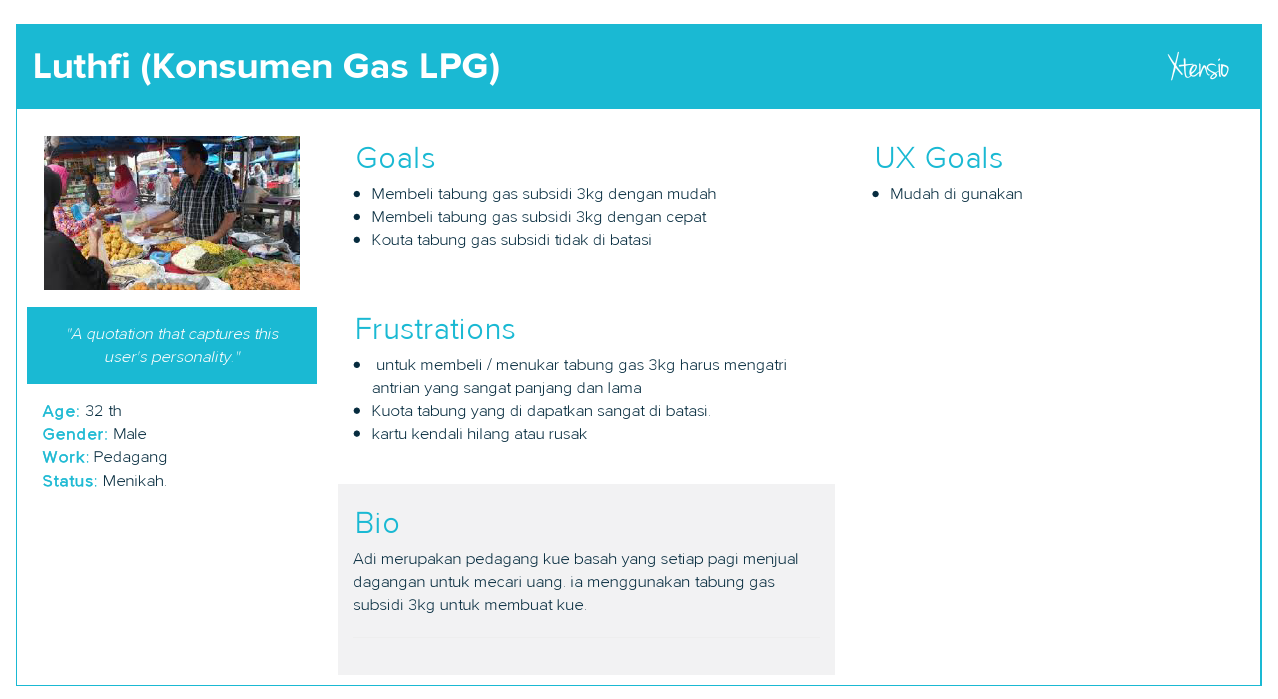
\includegraphics [width = 15cm]{gambar/persona/konsumen}
\end{figure}

\begin{figure}[H]
	\center
	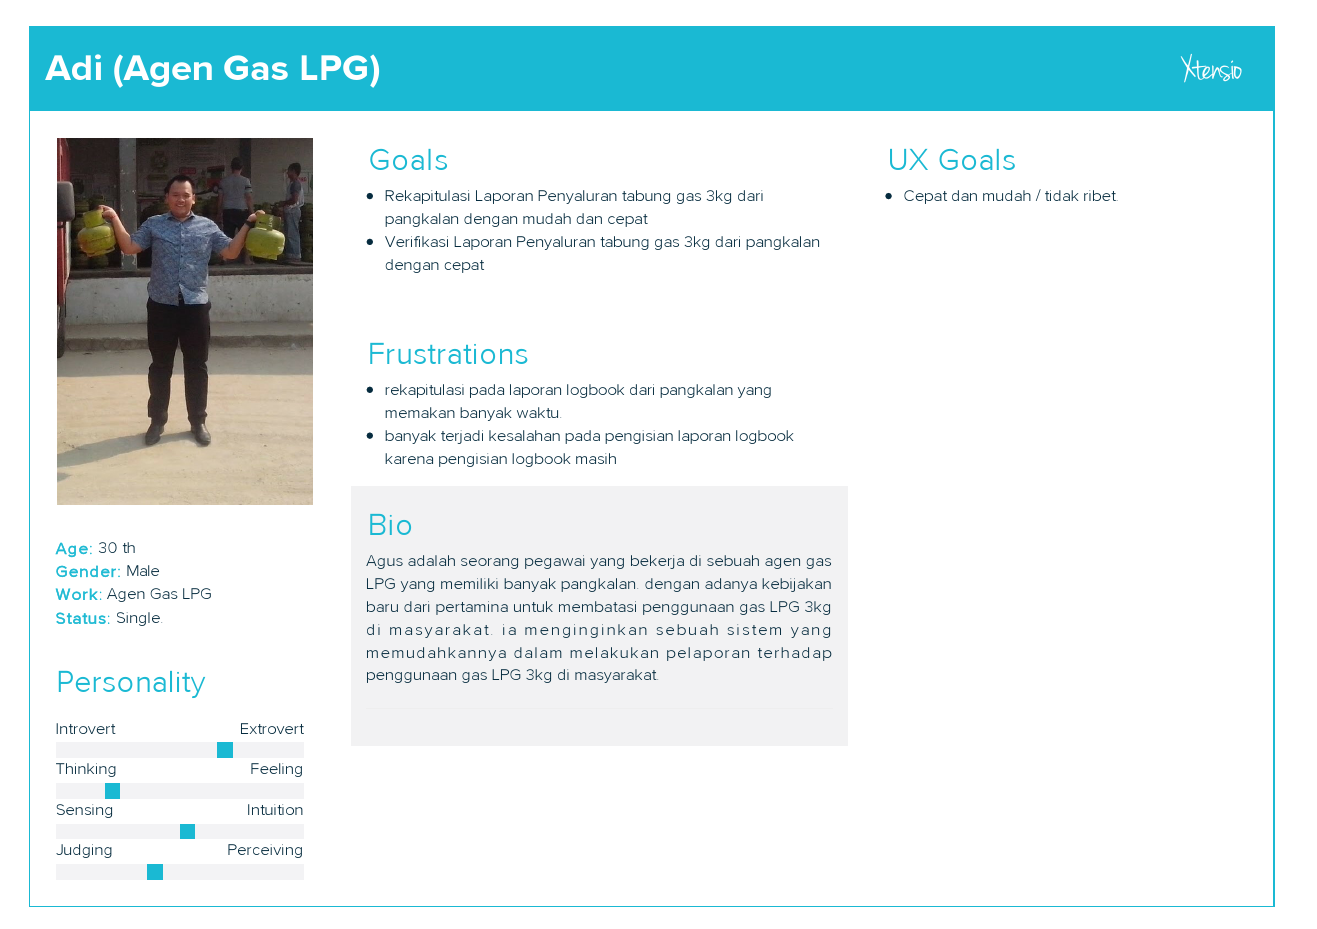
\includegraphics [width = 15cm]{gambar/persona/agen}
\end{figure}

\begin{figure}[H]
	\center
	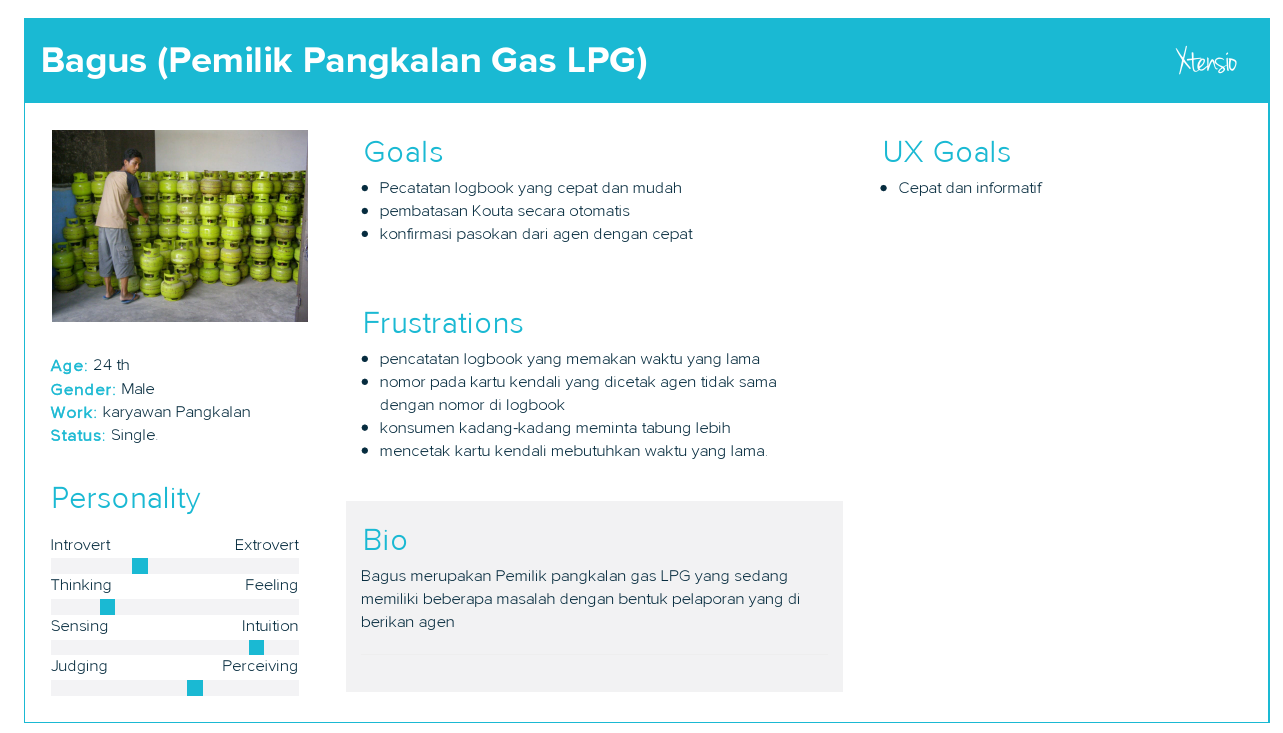
\includegraphics [width = 15cm]{gambar/persona/pangkalan}
\end{figure}
%-----------------------------------------------------------------------------%
\addcontentsline{toc}{chapter}{LAMPIRAN 2}
\chapter*{Lampiran 2}
\newappendix{Lampiran 2. Kuesioner SUS}
\begin{figure}[H]
	\center
	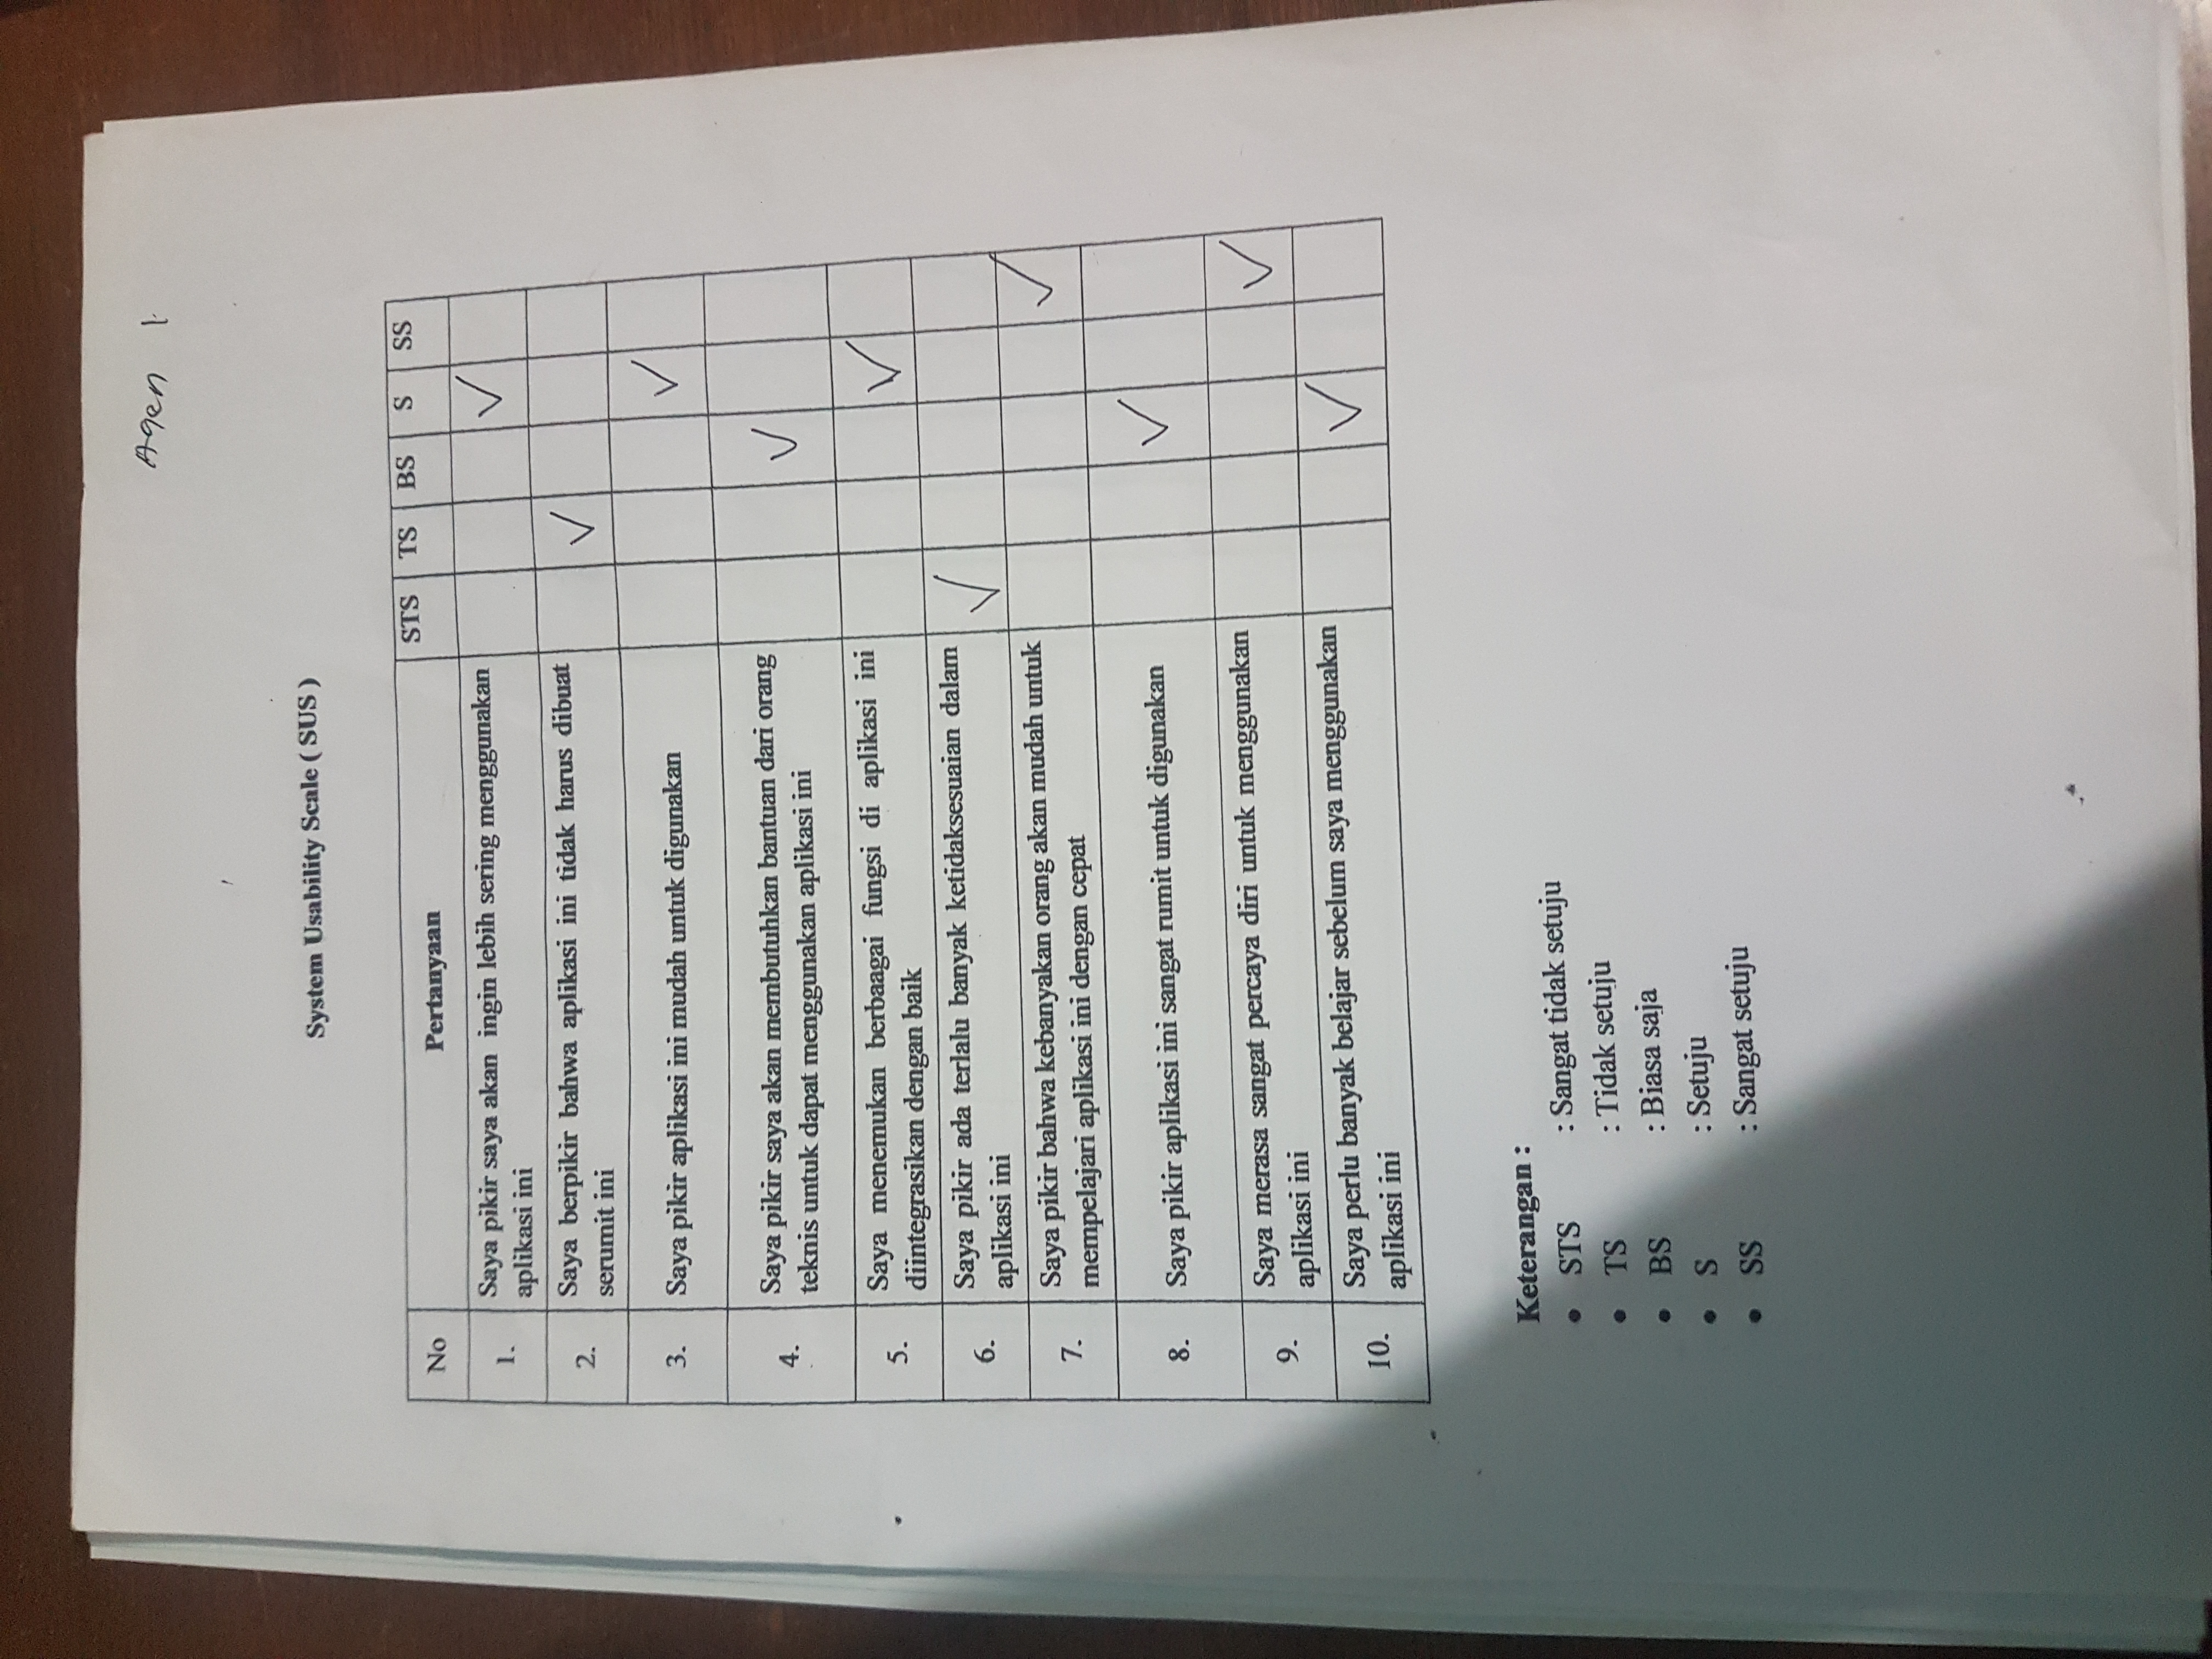
\includegraphics [width = 17cm,angle=-90]{gambar/pengujian/agen1}
\end{figure}
\begin{figure}[H]
	\center
	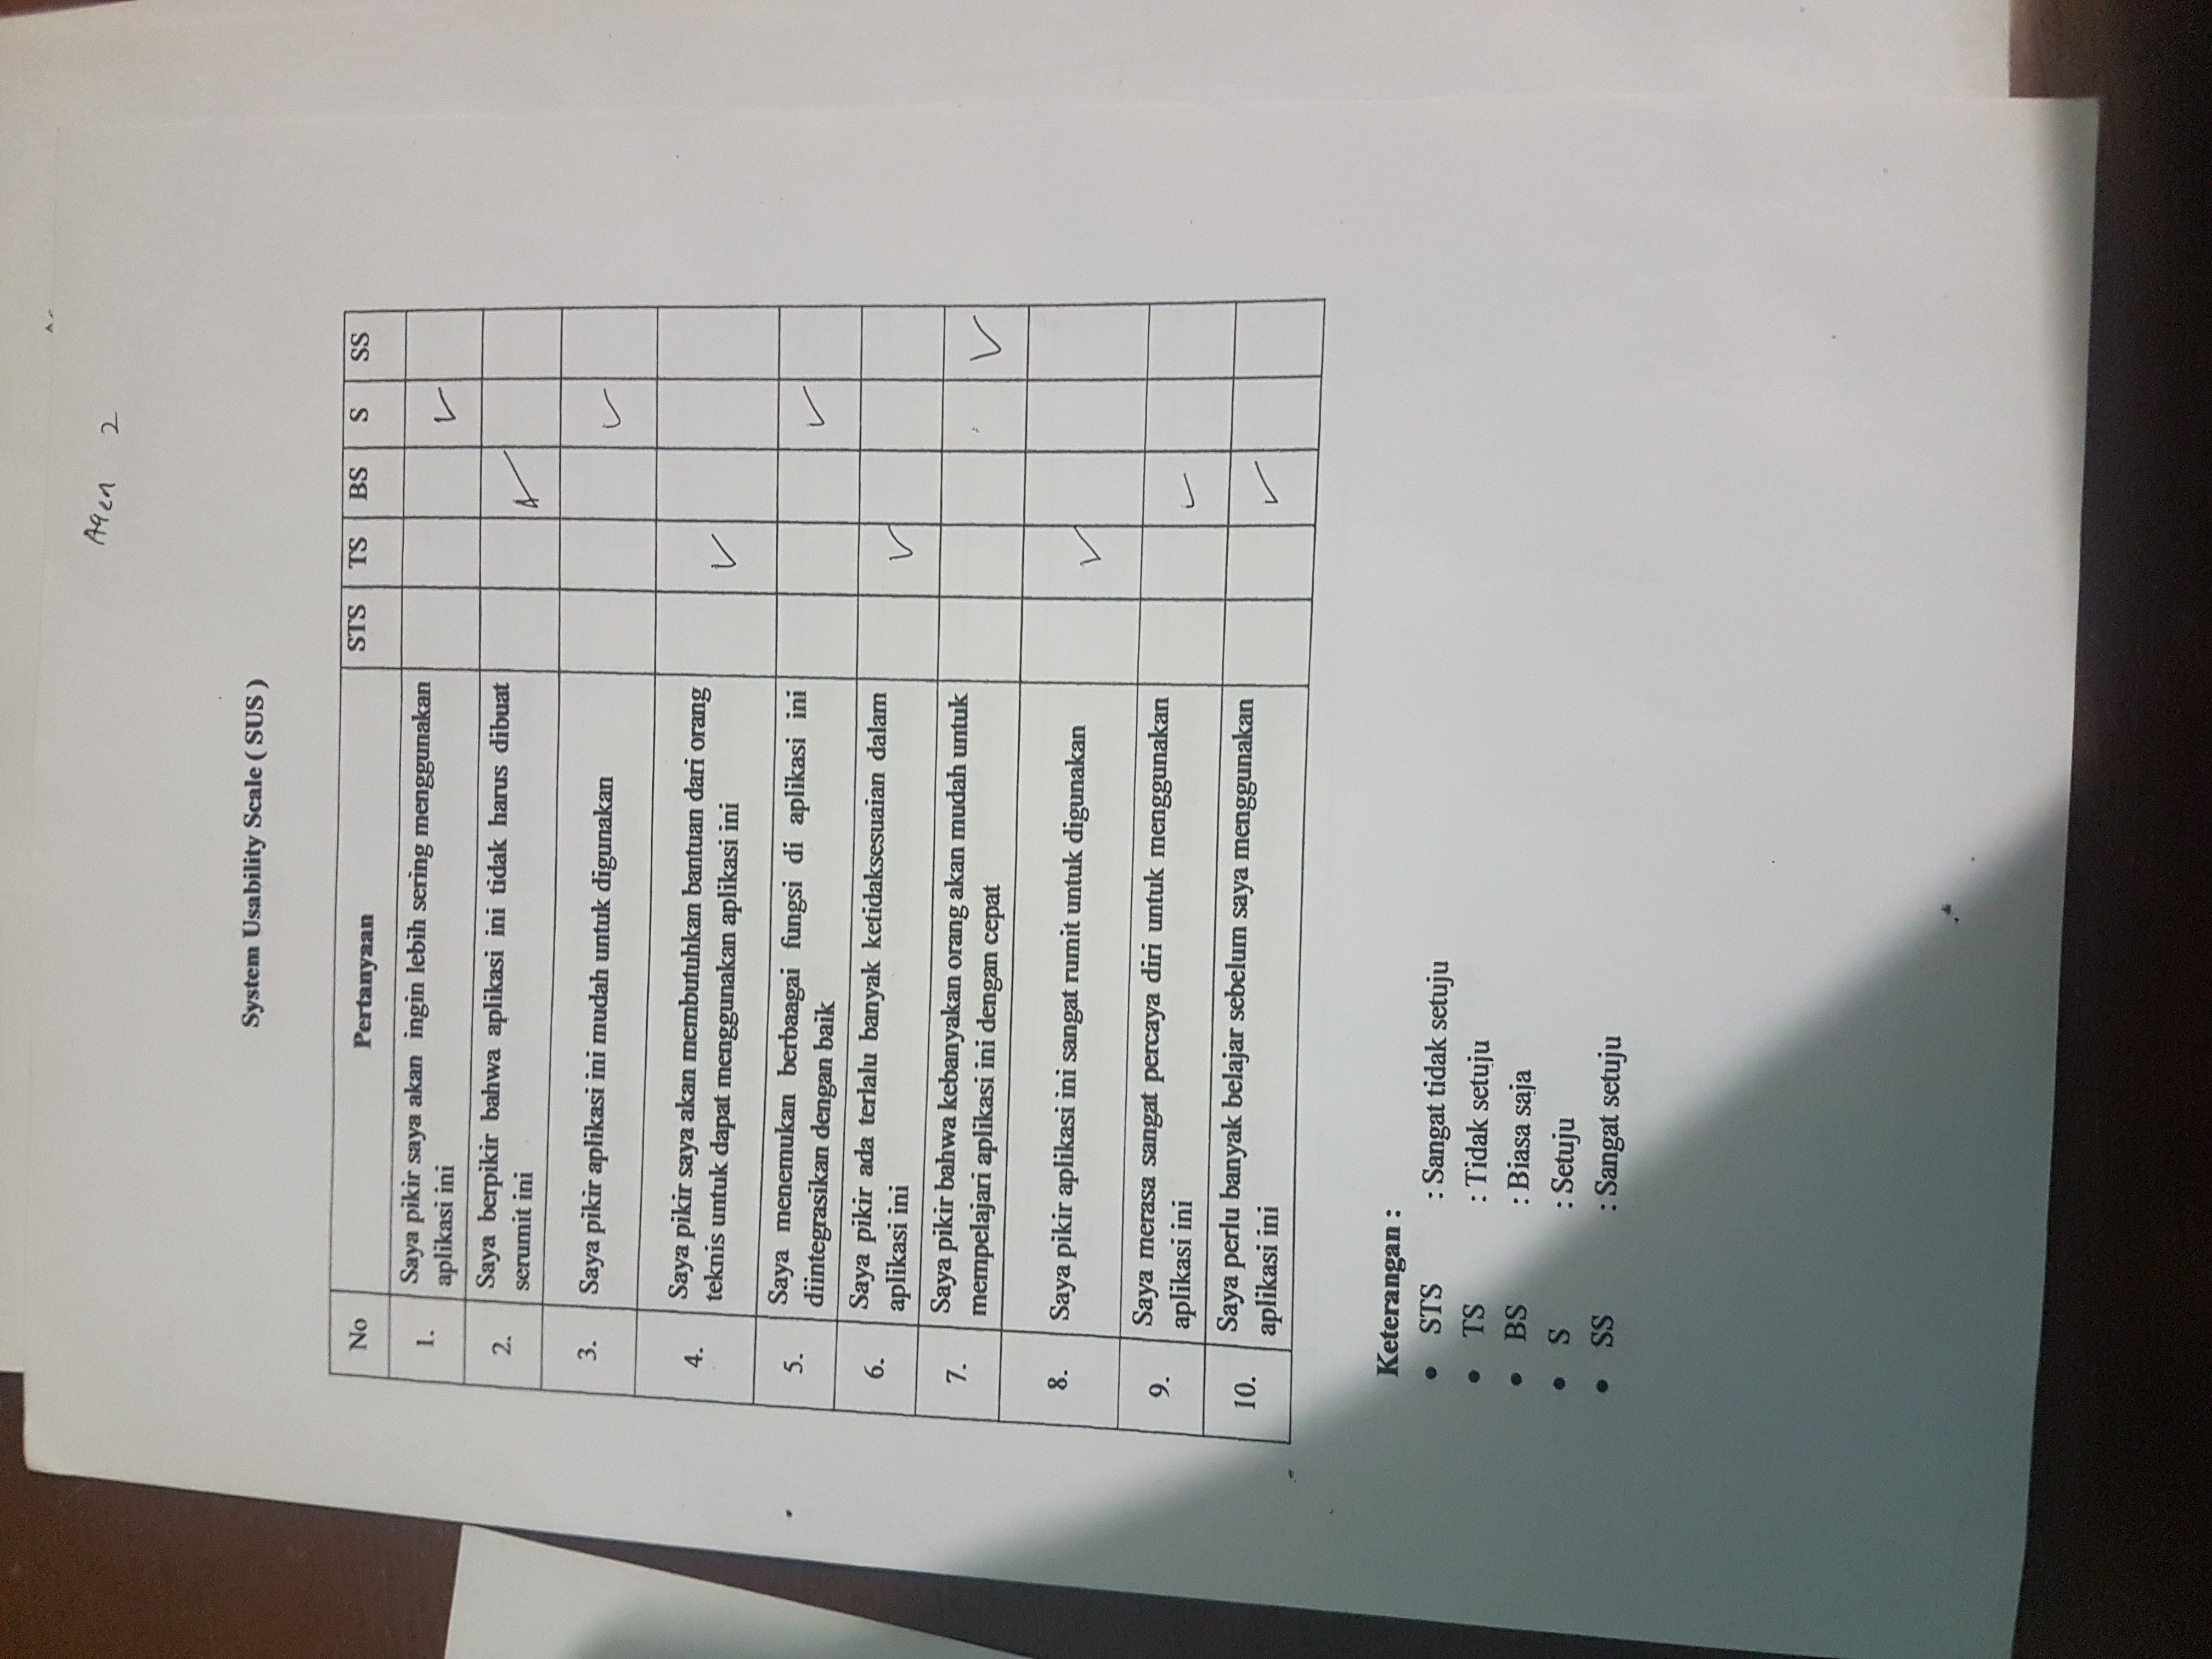
\includegraphics [width = 17cm,angle=-90]{gambar/pengujian/agen2}
\end{figure}
\begin{figure}[H]
	\center
	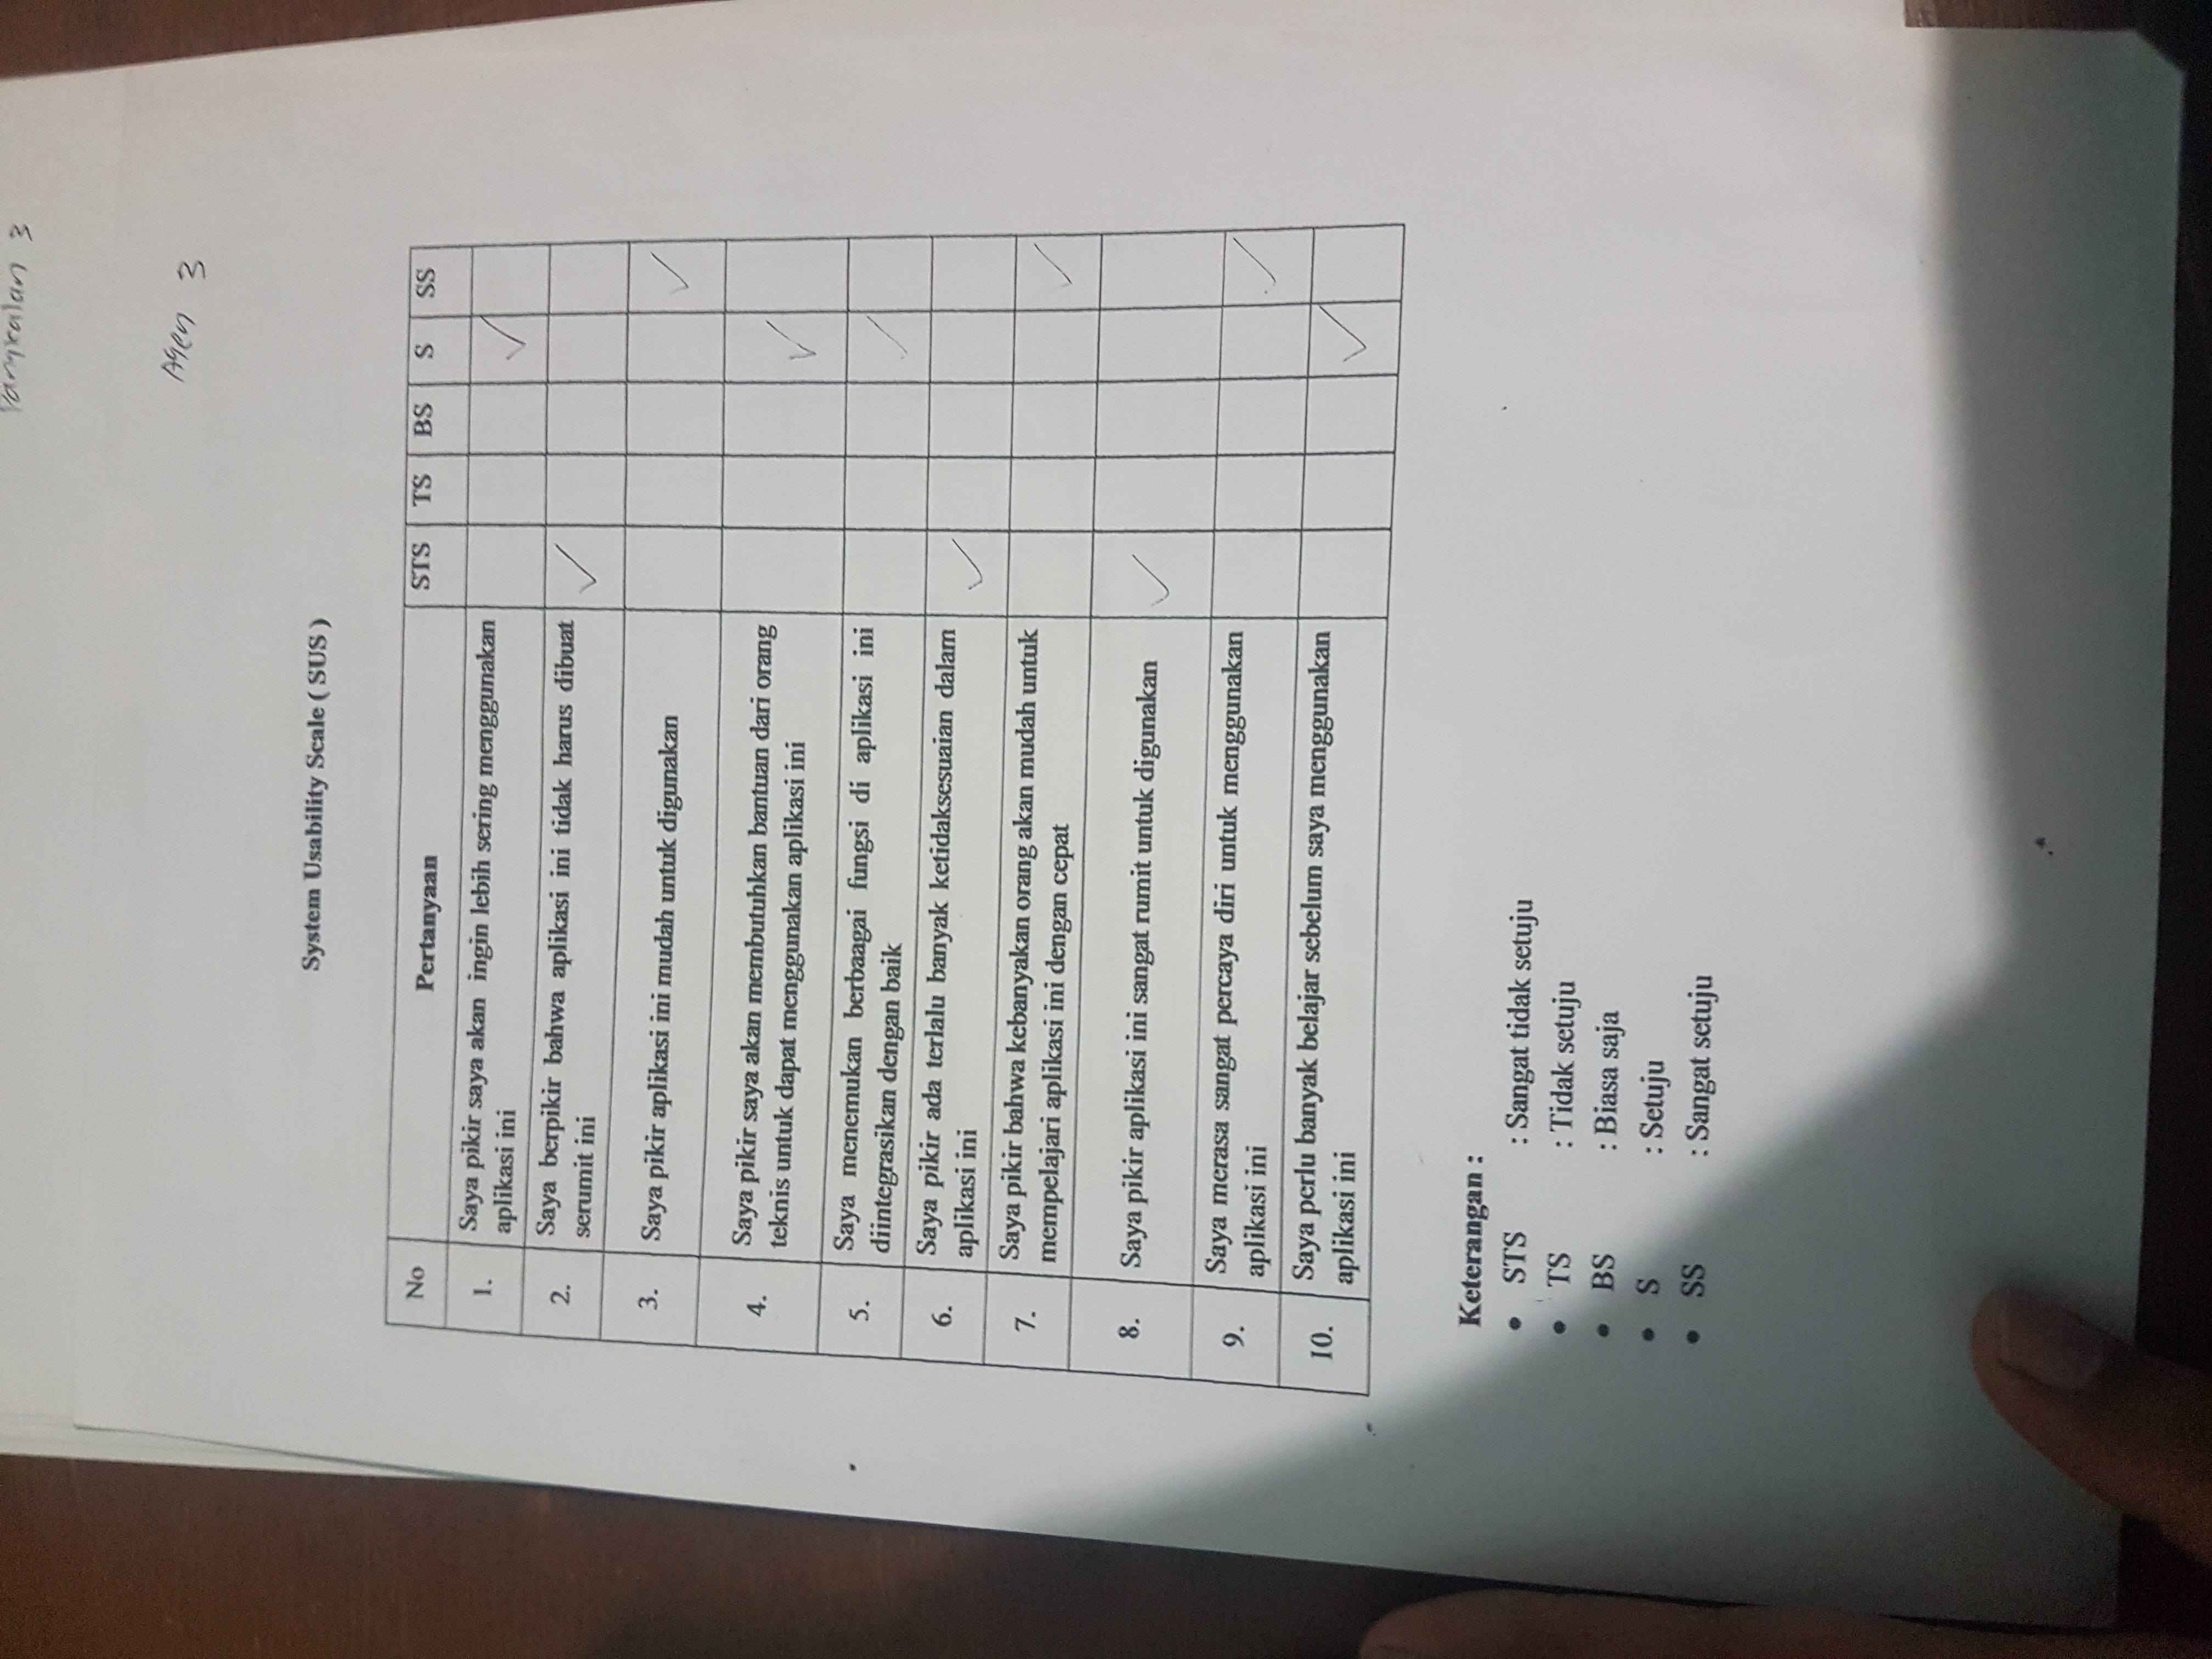
\includegraphics [width = 17cm,angle=-90]{gambar/pengujian/agen3}
\end{figure}
\begin{figure}[H]
	\center
	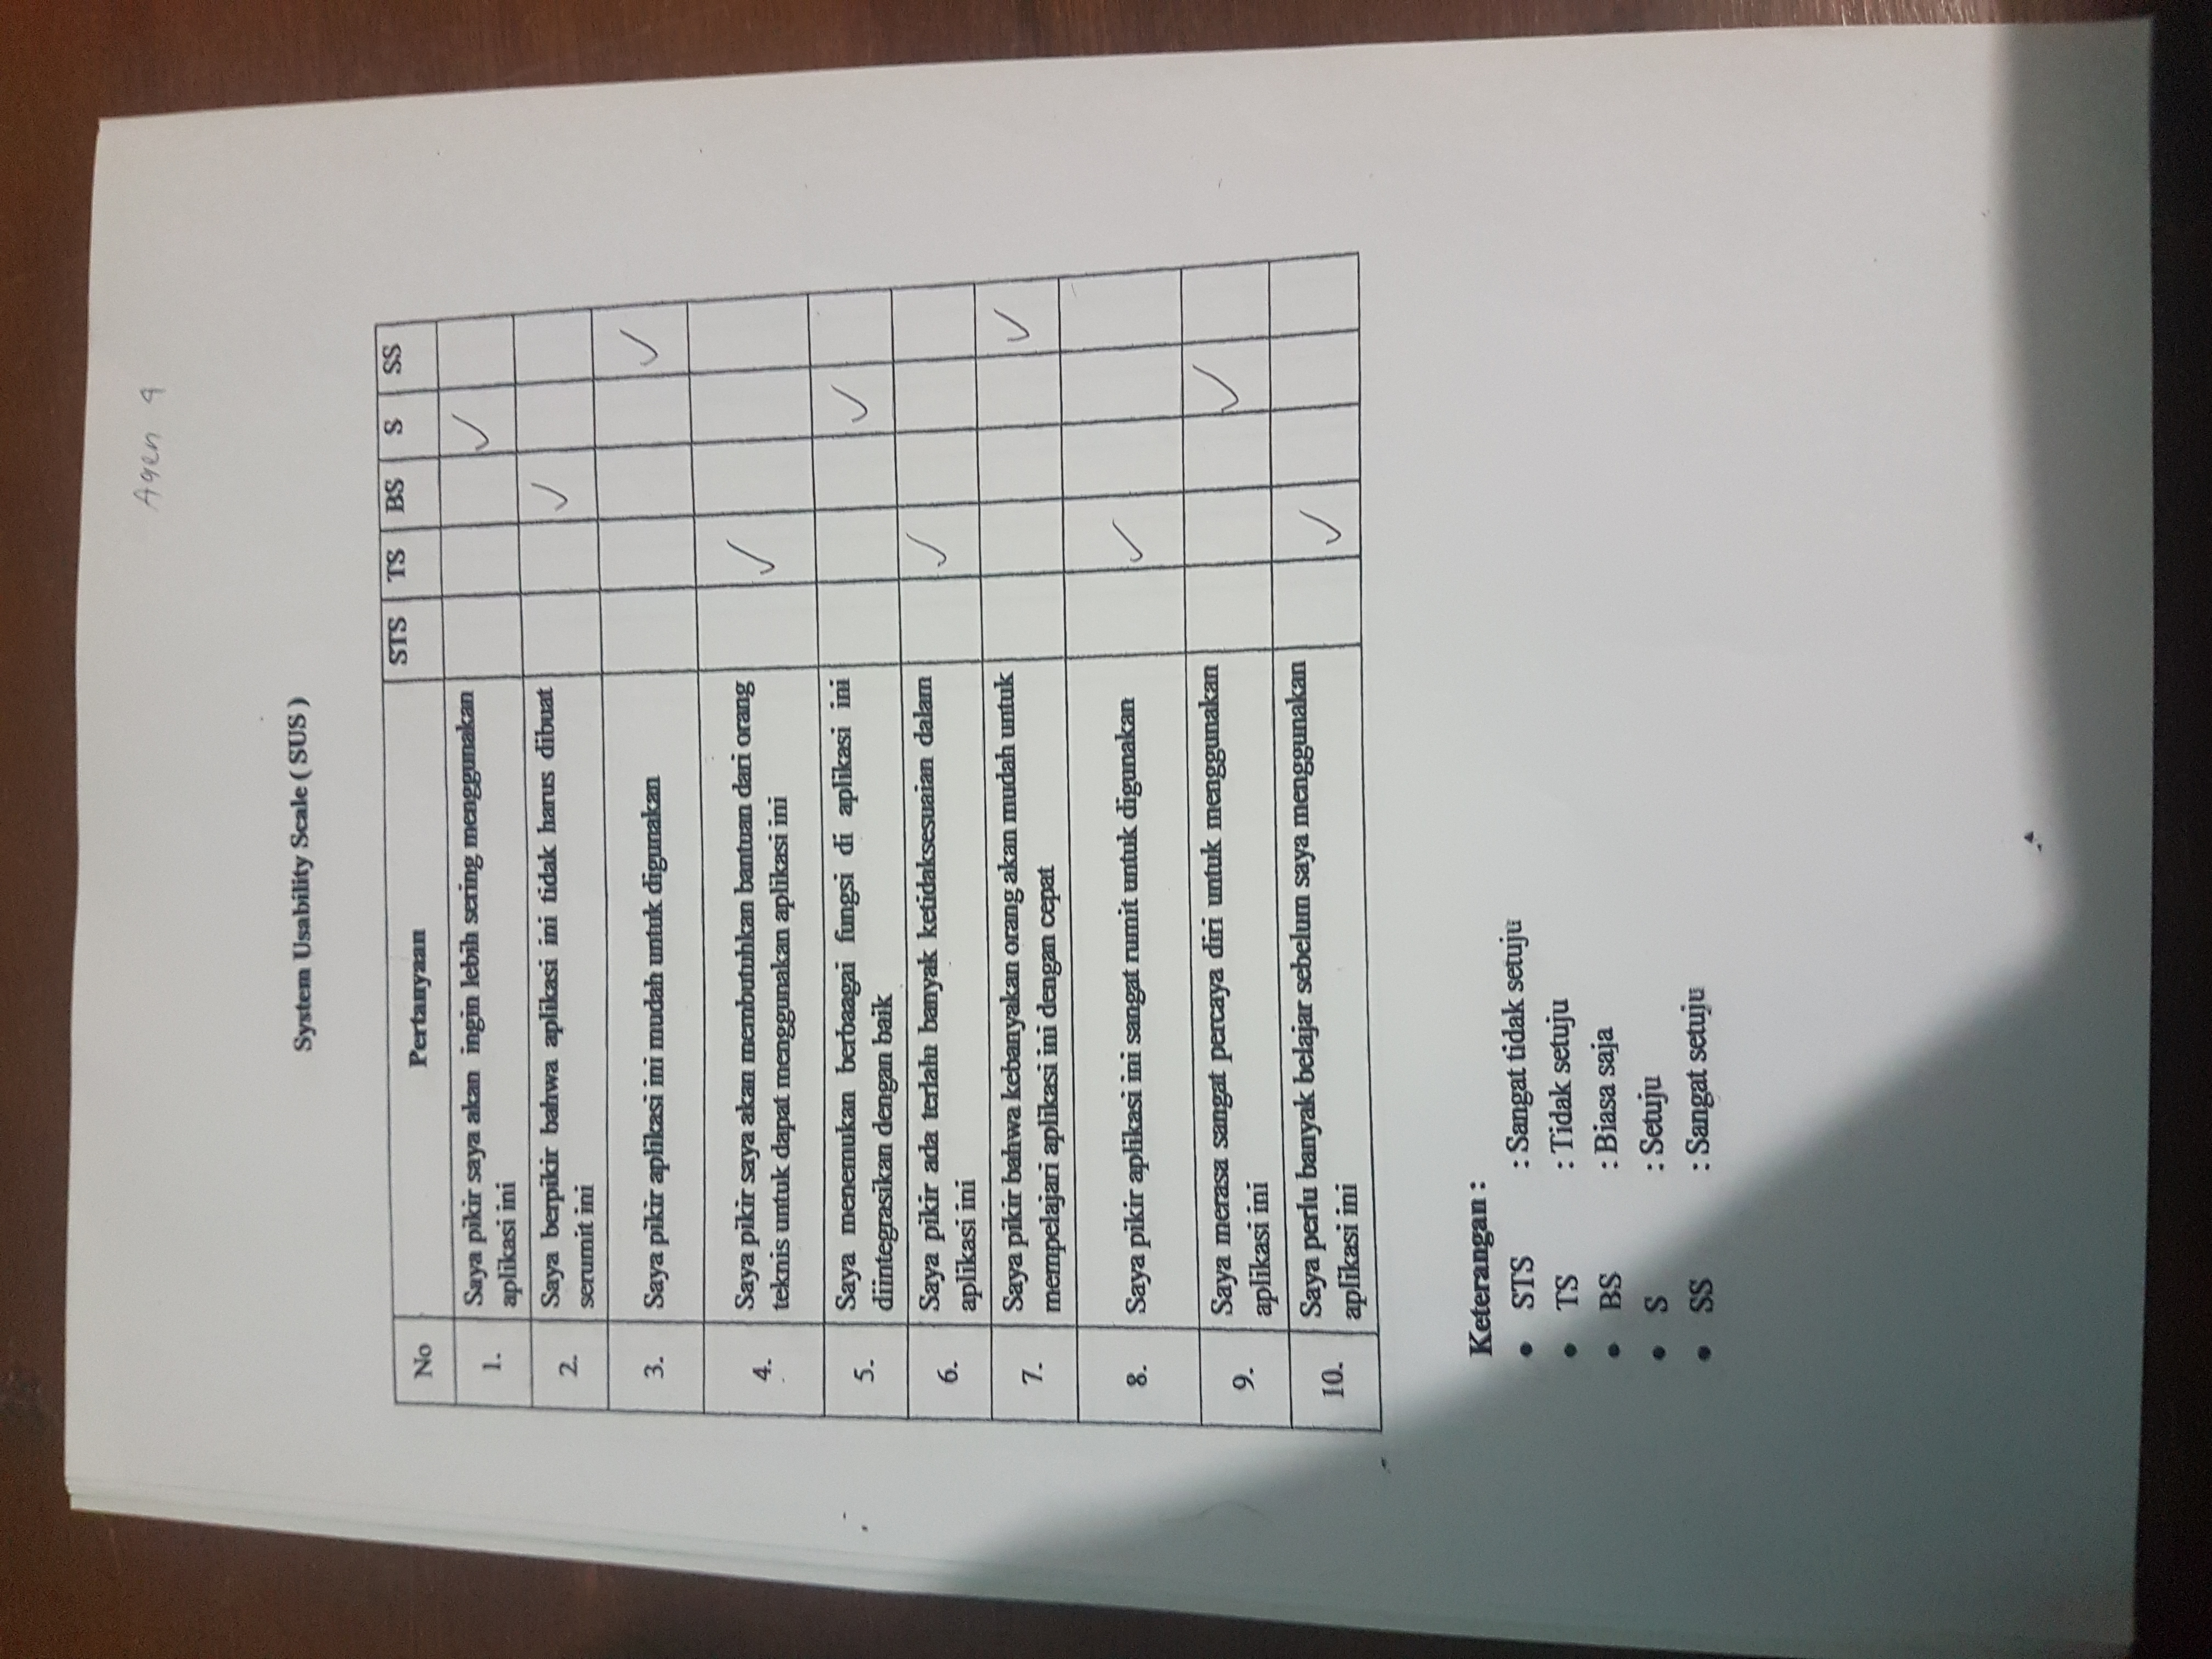
\includegraphics [width = 17cm,angle=-90]{gambar/pengujian/agen4}
\end{figure}
\begin{figure}[H]
	\center
	\includegraphics [width = 17cm,angle=-90]{gambar/pengujian/agen5}
\end{figure}
\begin{figure}[H]
	\center
	\includegraphics [width = 17cm,angle=-90]{gambar/pengujian/agen6}
\end{figure}
\begin{figure}[H]
	\center
	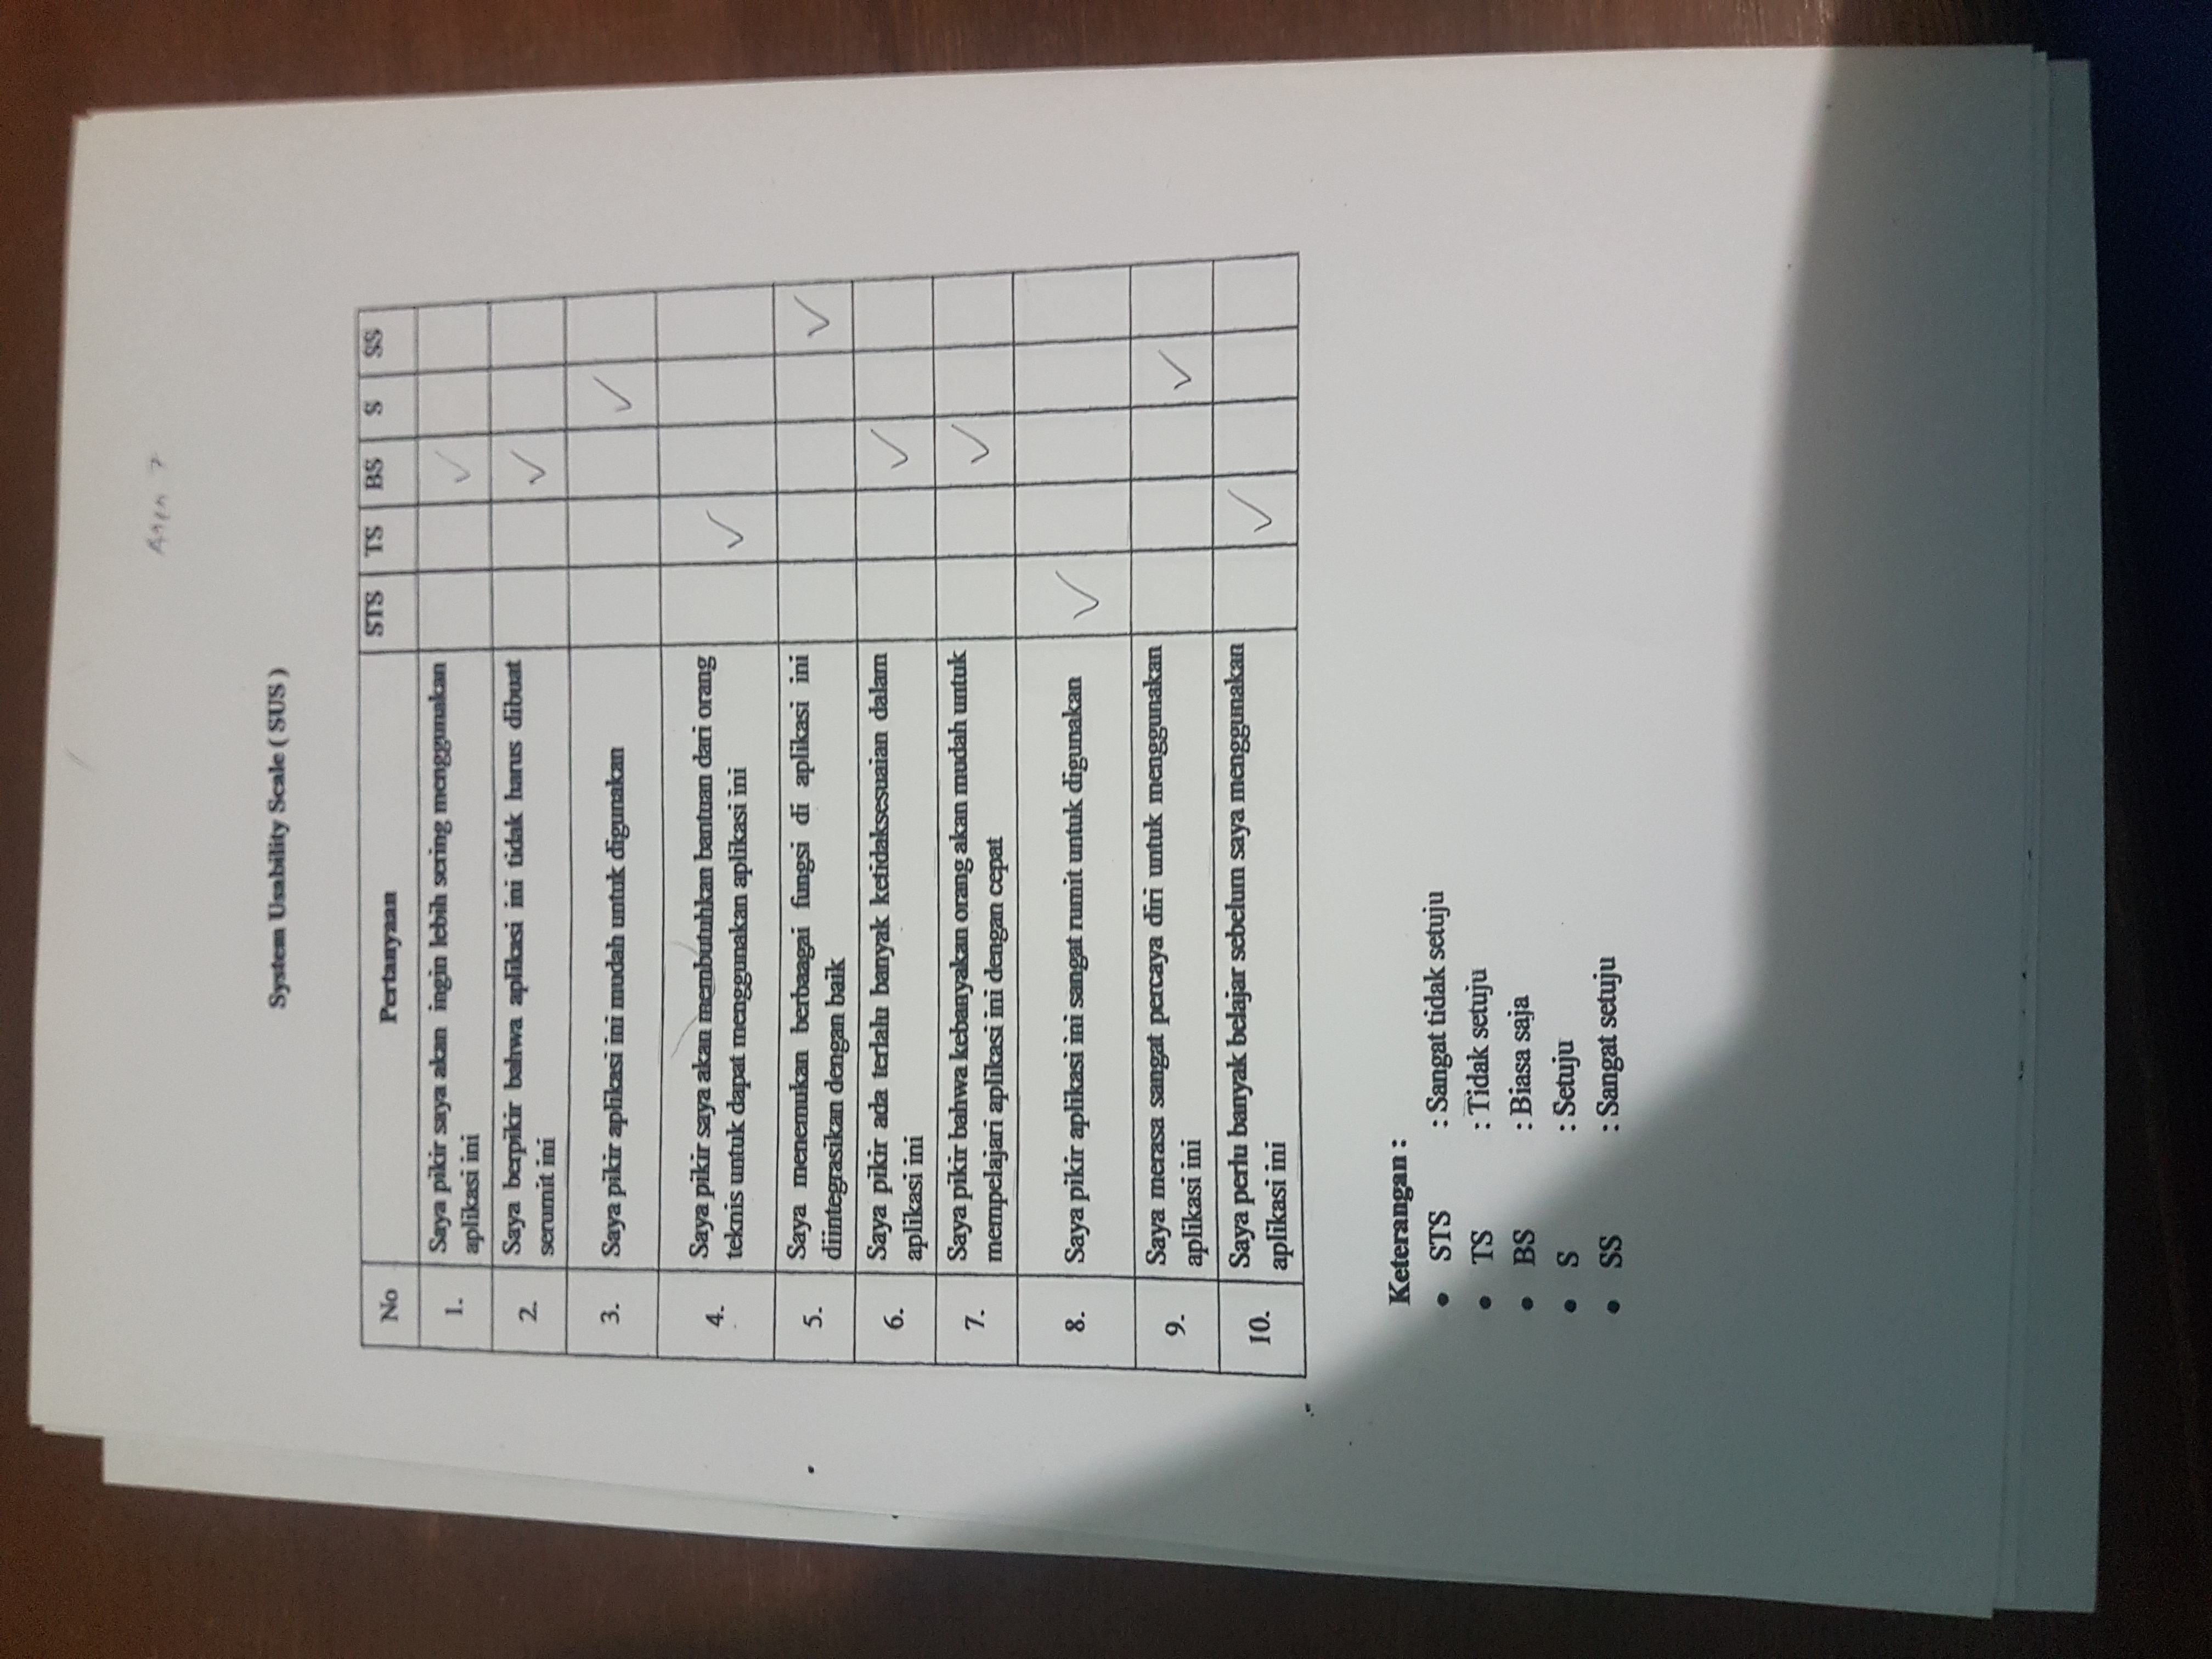
\includegraphics [width = 17cm,angle=-90]{gambar/pengujian/agen7}
\end{figure}
\begin{figure}[H]
	\center
	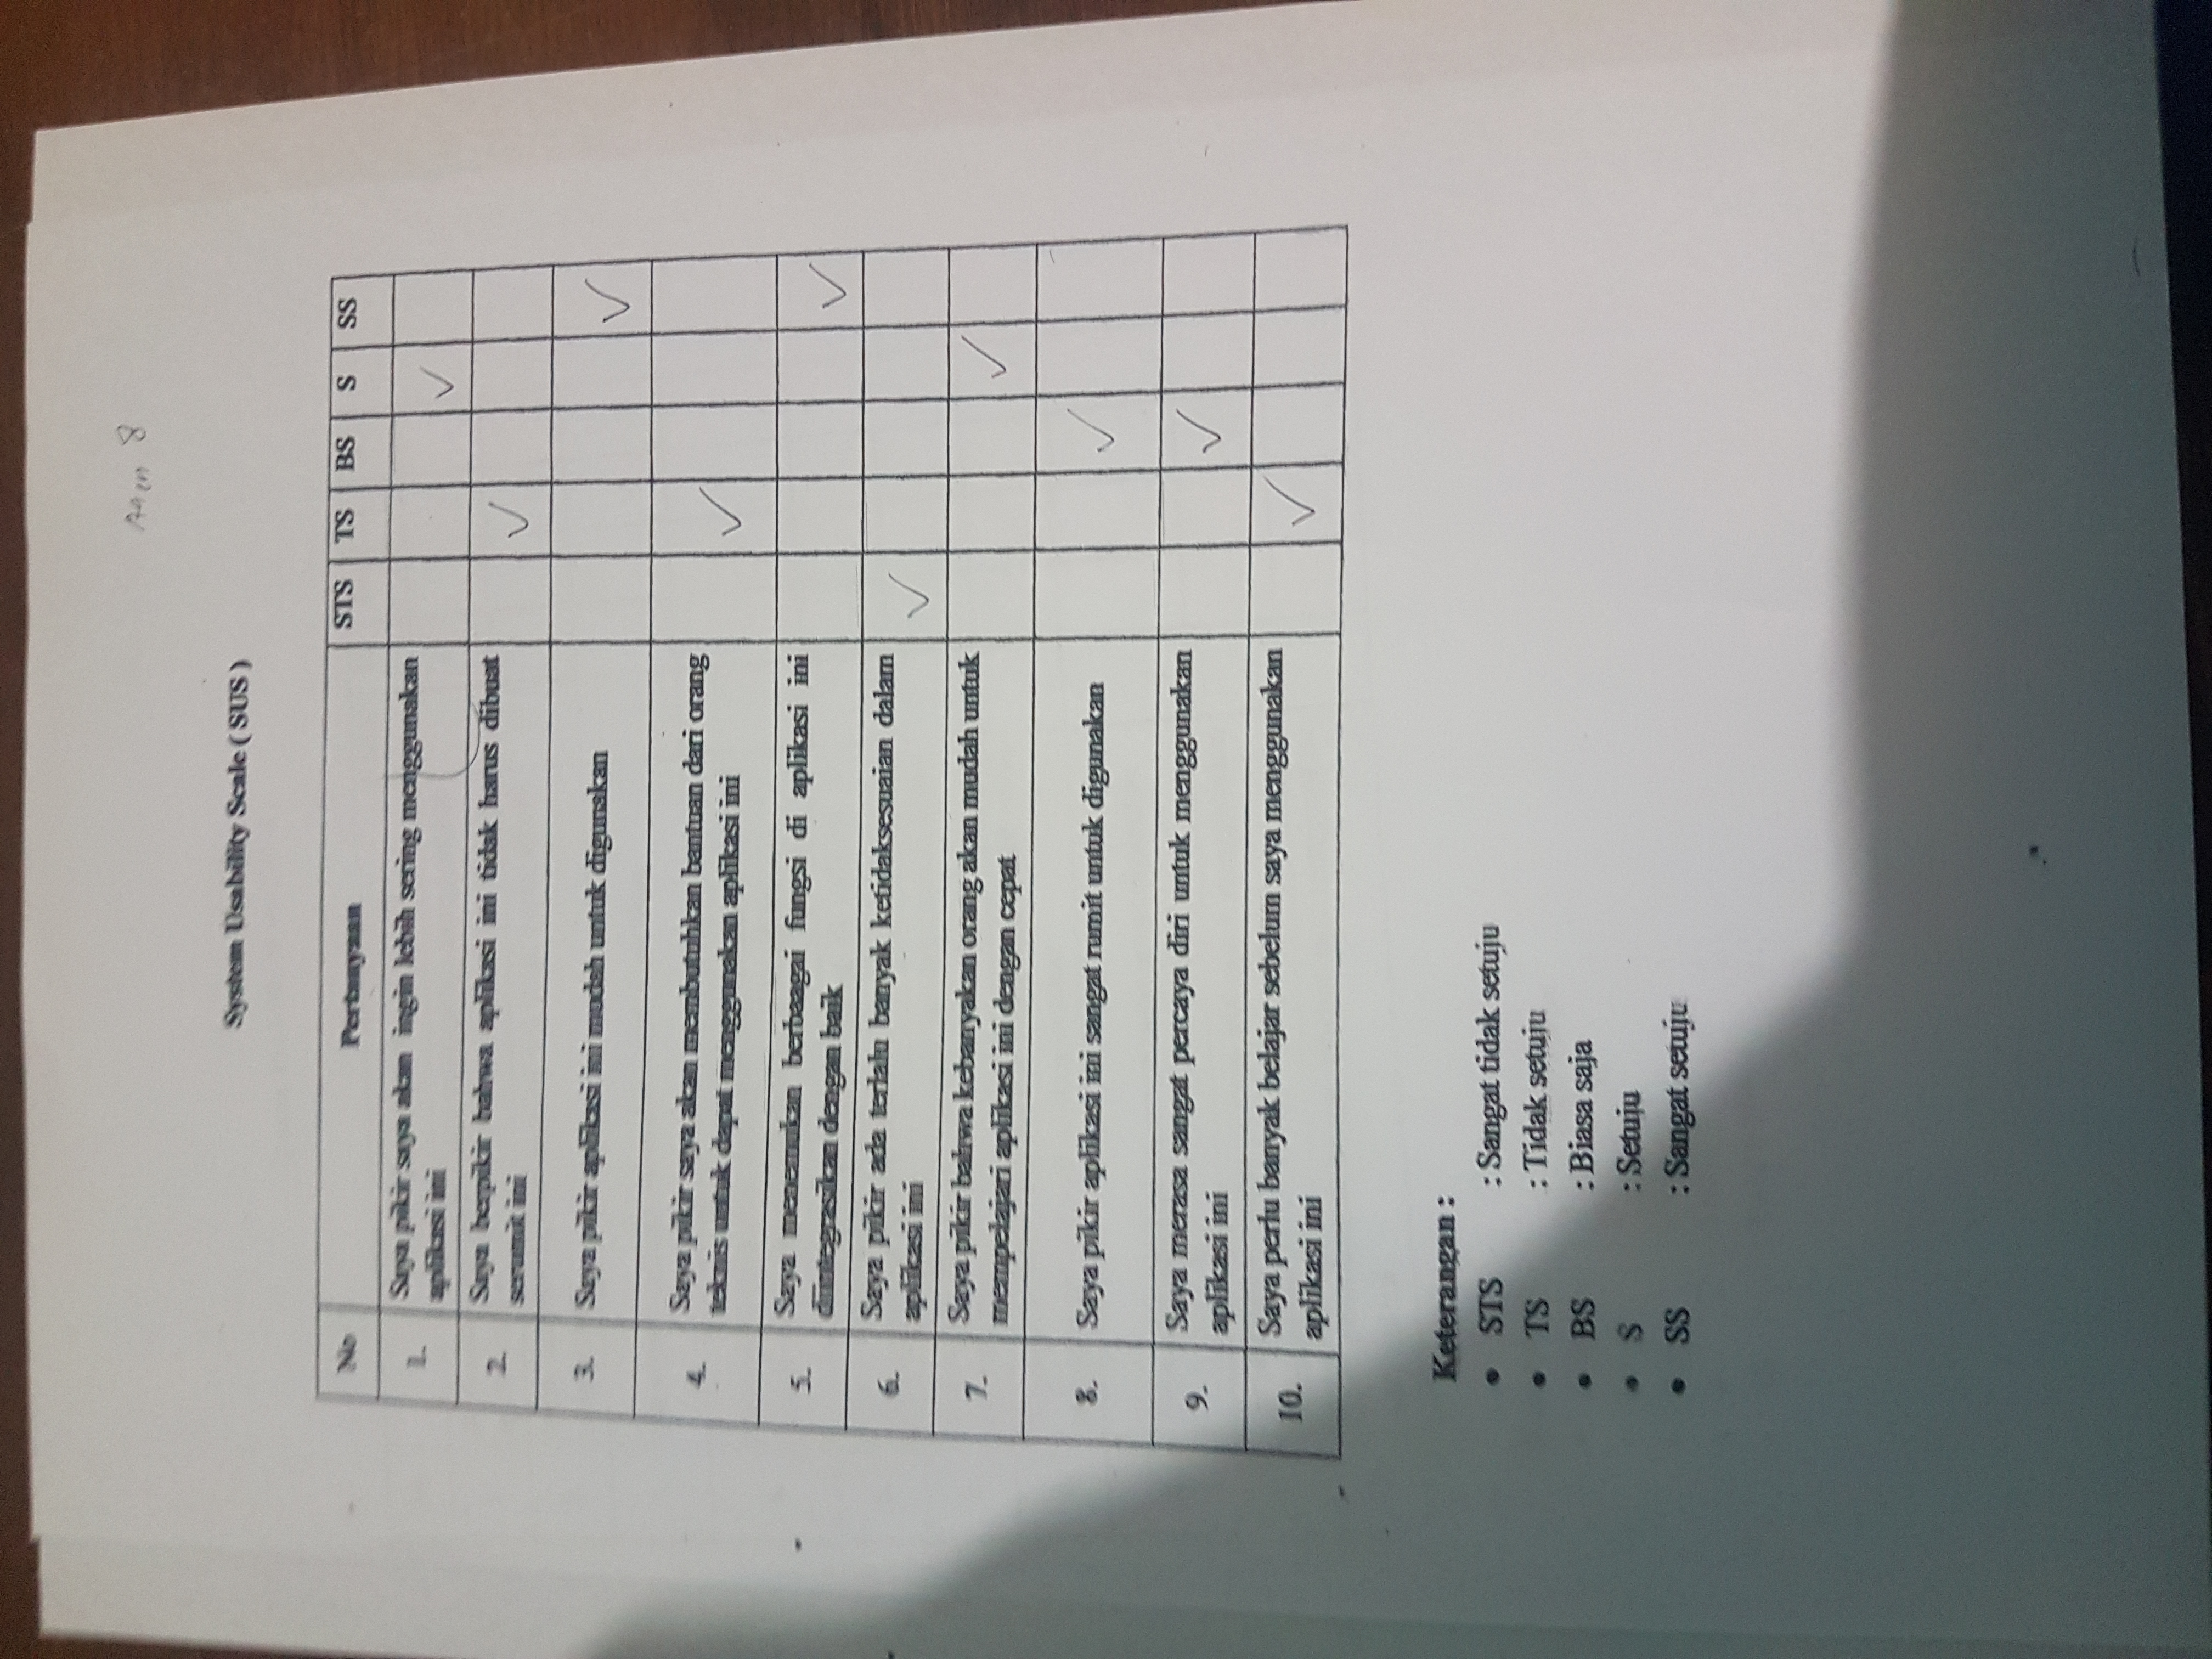
\includegraphics [width = 17cm,angle=-90]{gambar/pengujian/agen8}
\end{figure}

\begin{figure}[H]
	\center
	\includegraphics [width = 17cm,angle=-90]{gambar/pengujian/pangkalan1}
\end{figure}

\begin{figure}[H]
	\center
	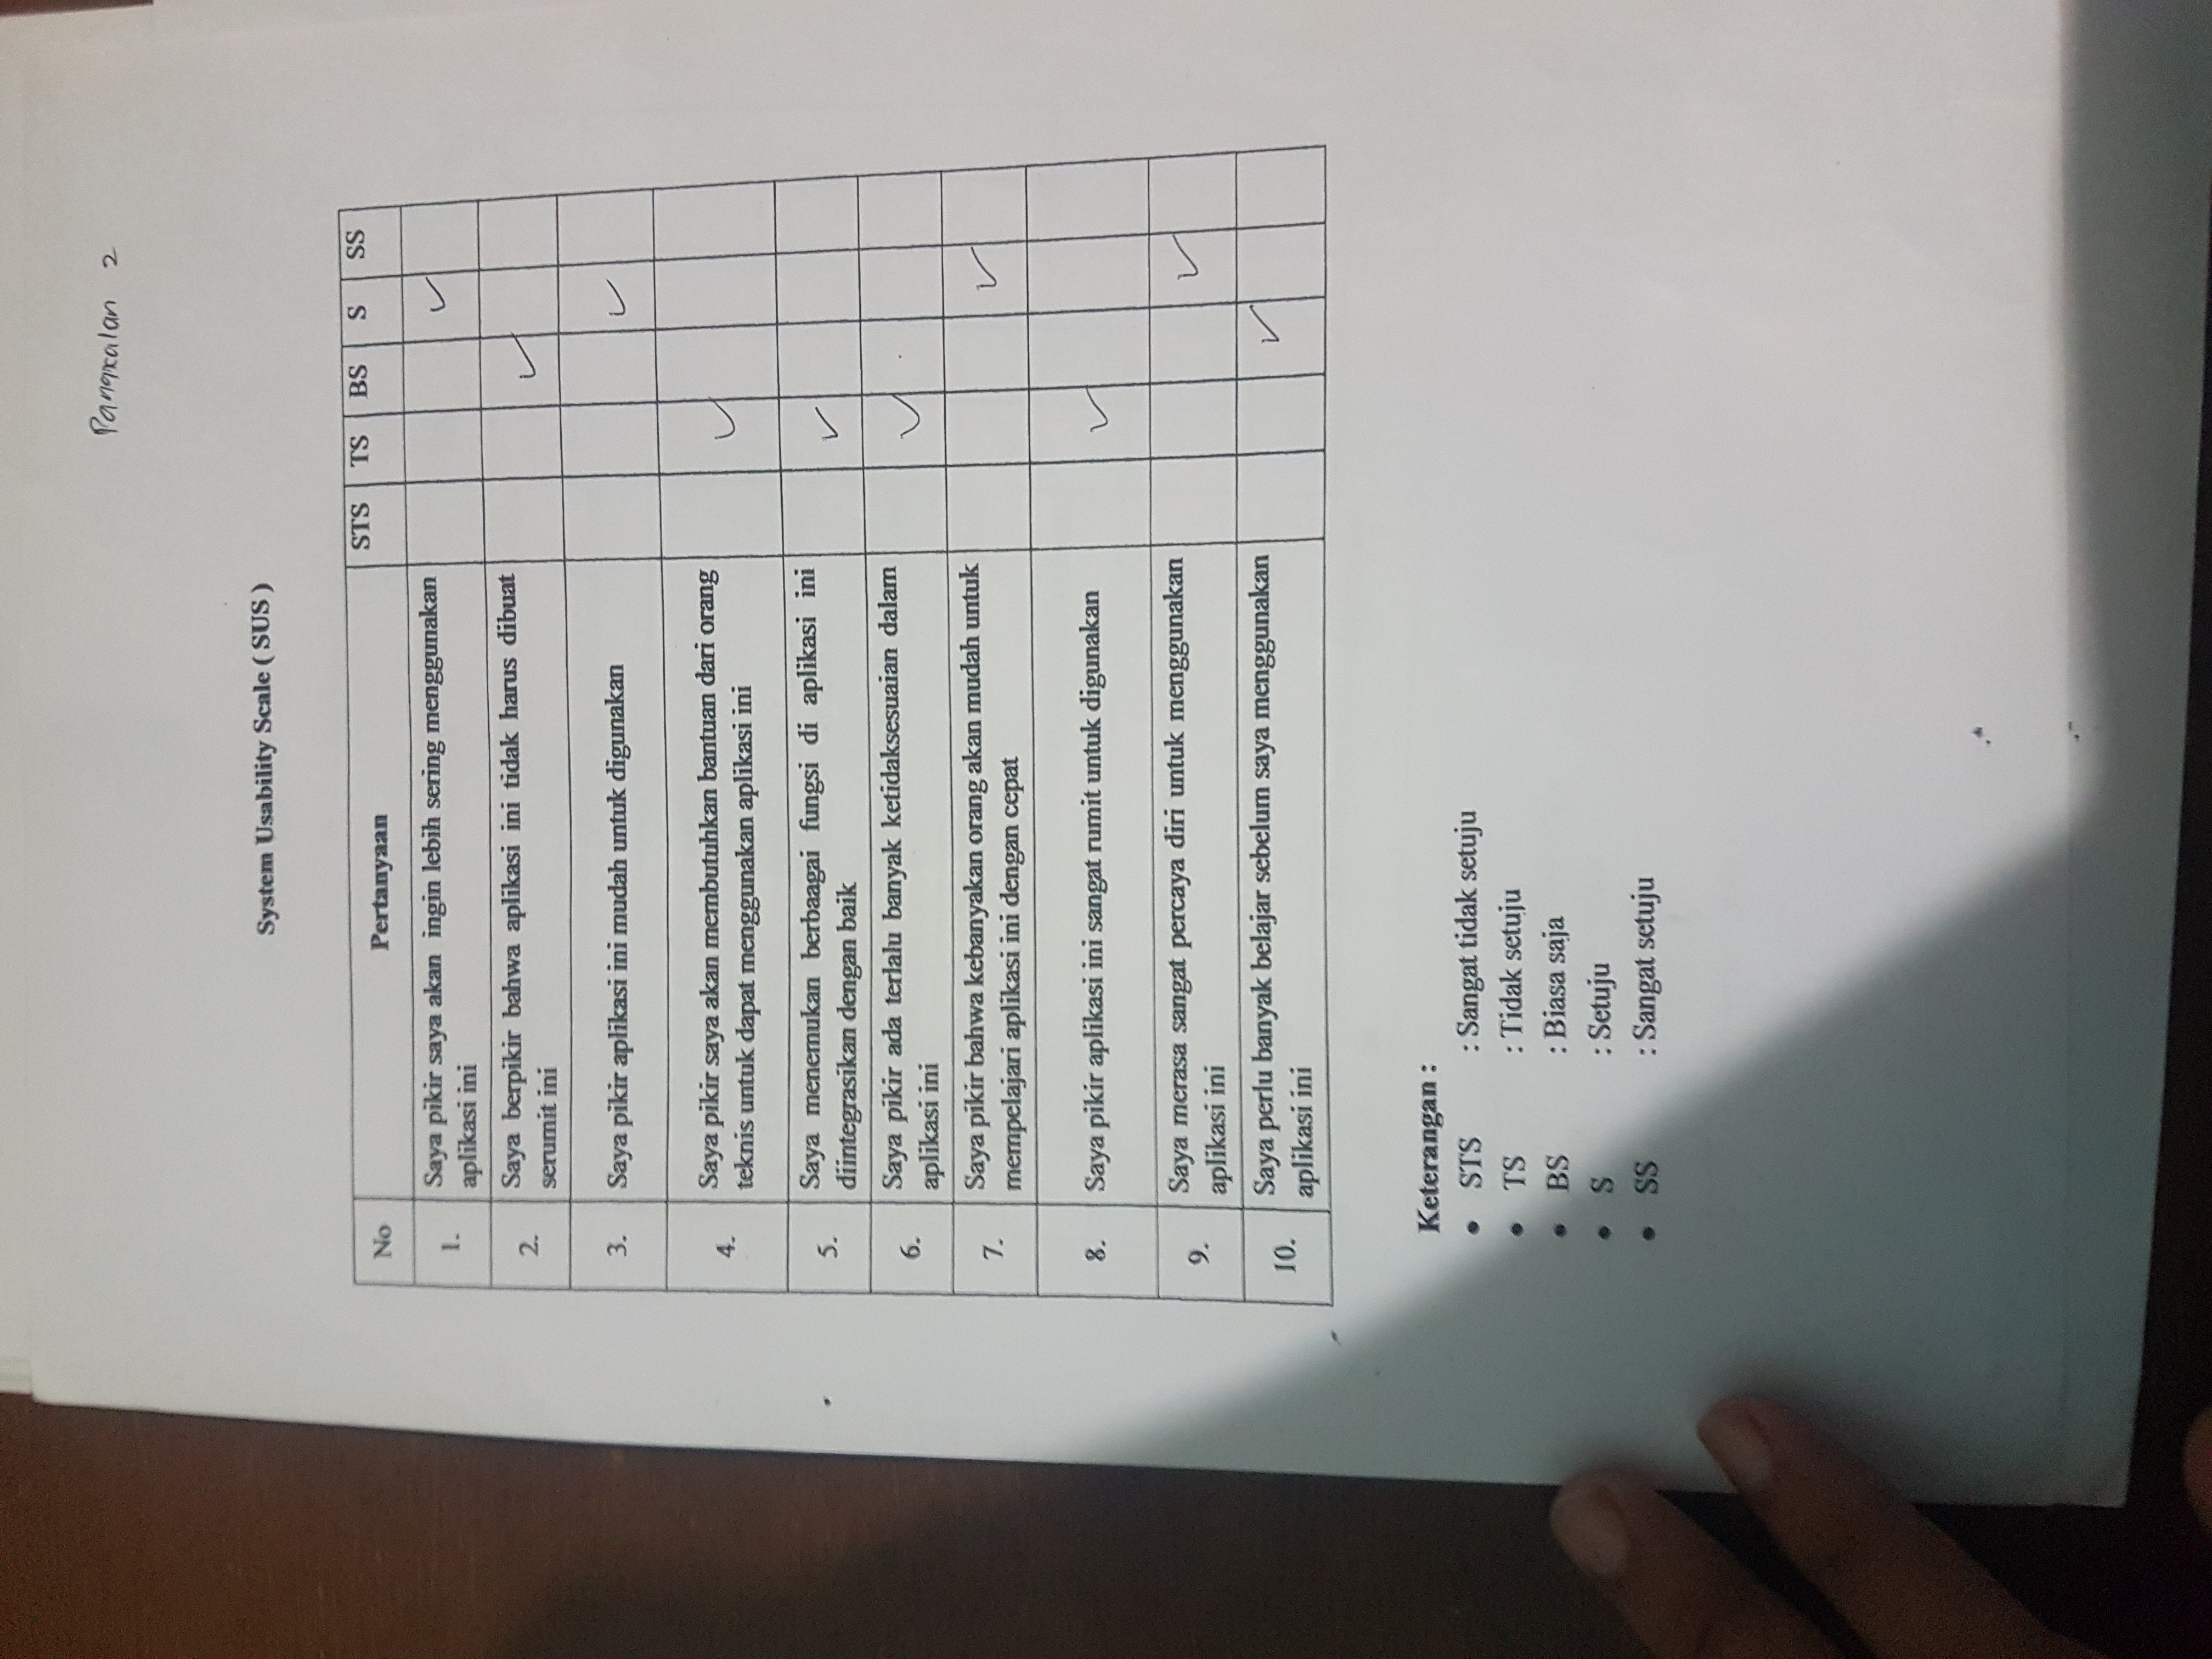
\includegraphics [width = 17cm,angle=-90]{gambar/pengujian/pangkalan2}
\end{figure}
\begin{figure}[H]
	\center
	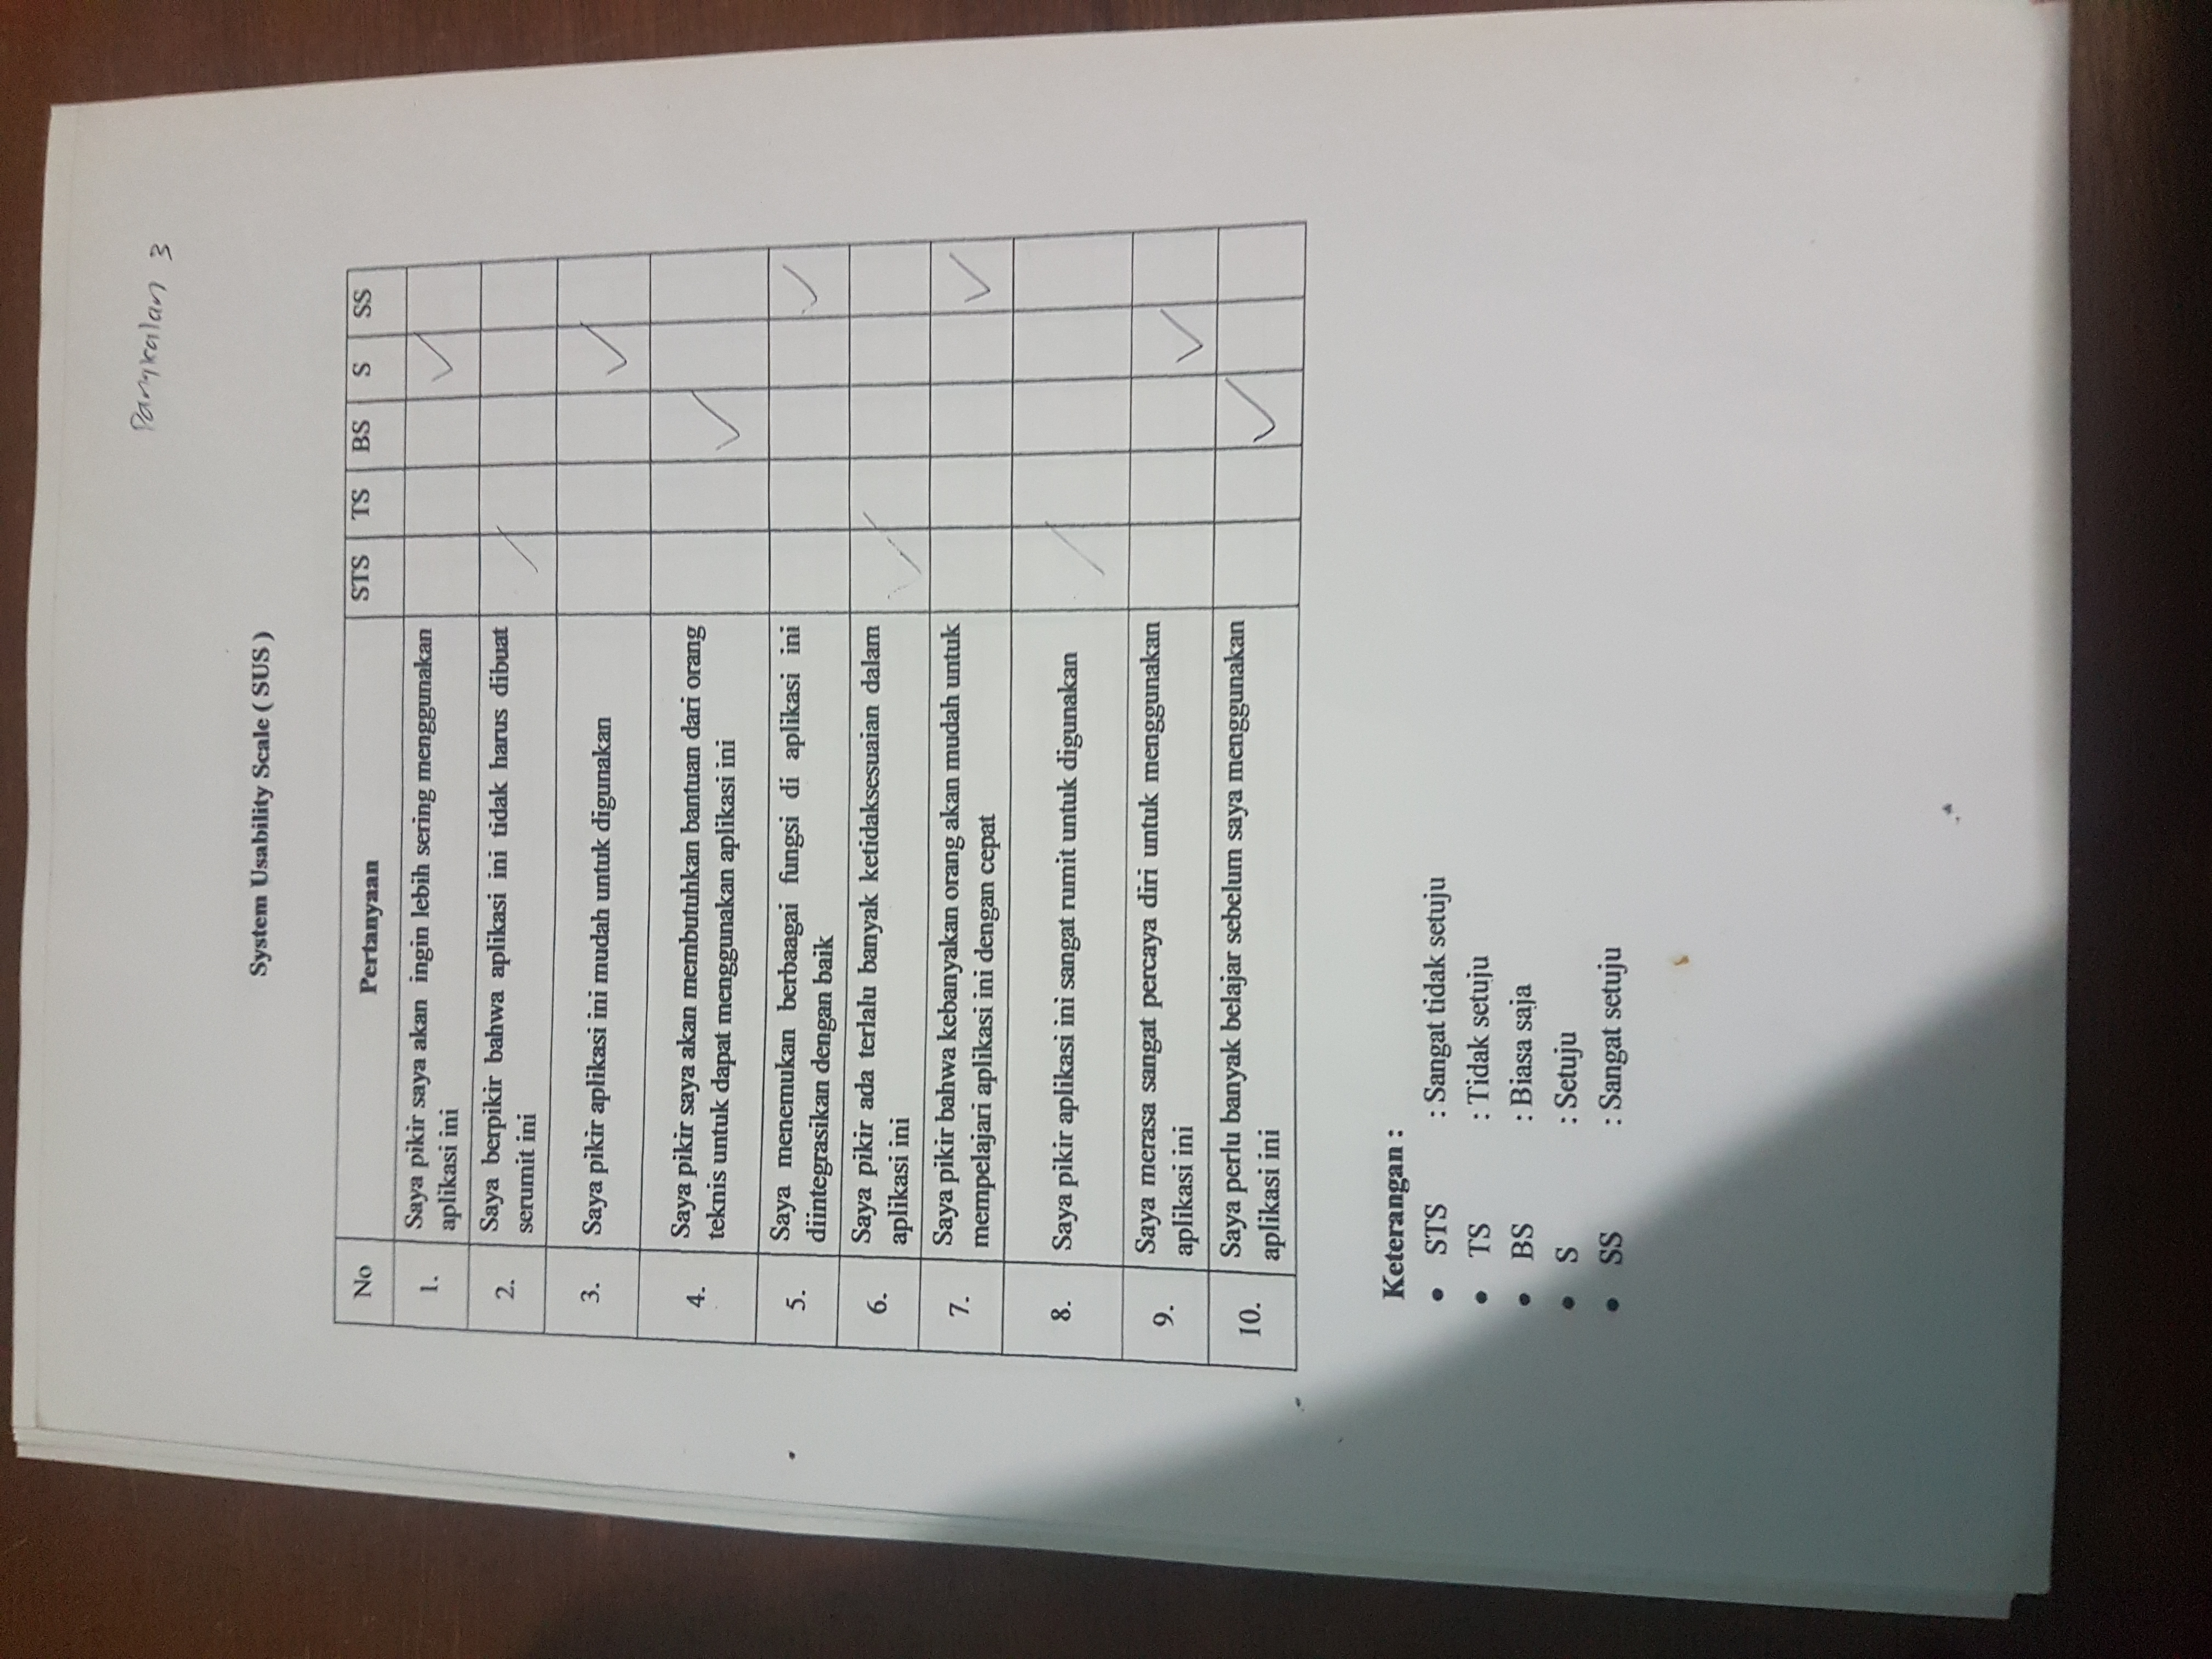
\includegraphics [width = 17cm,angle=-90]{gambar/pengujian/pangkalan3}
\end{figure}
\begin{figure}[H]
	\center
	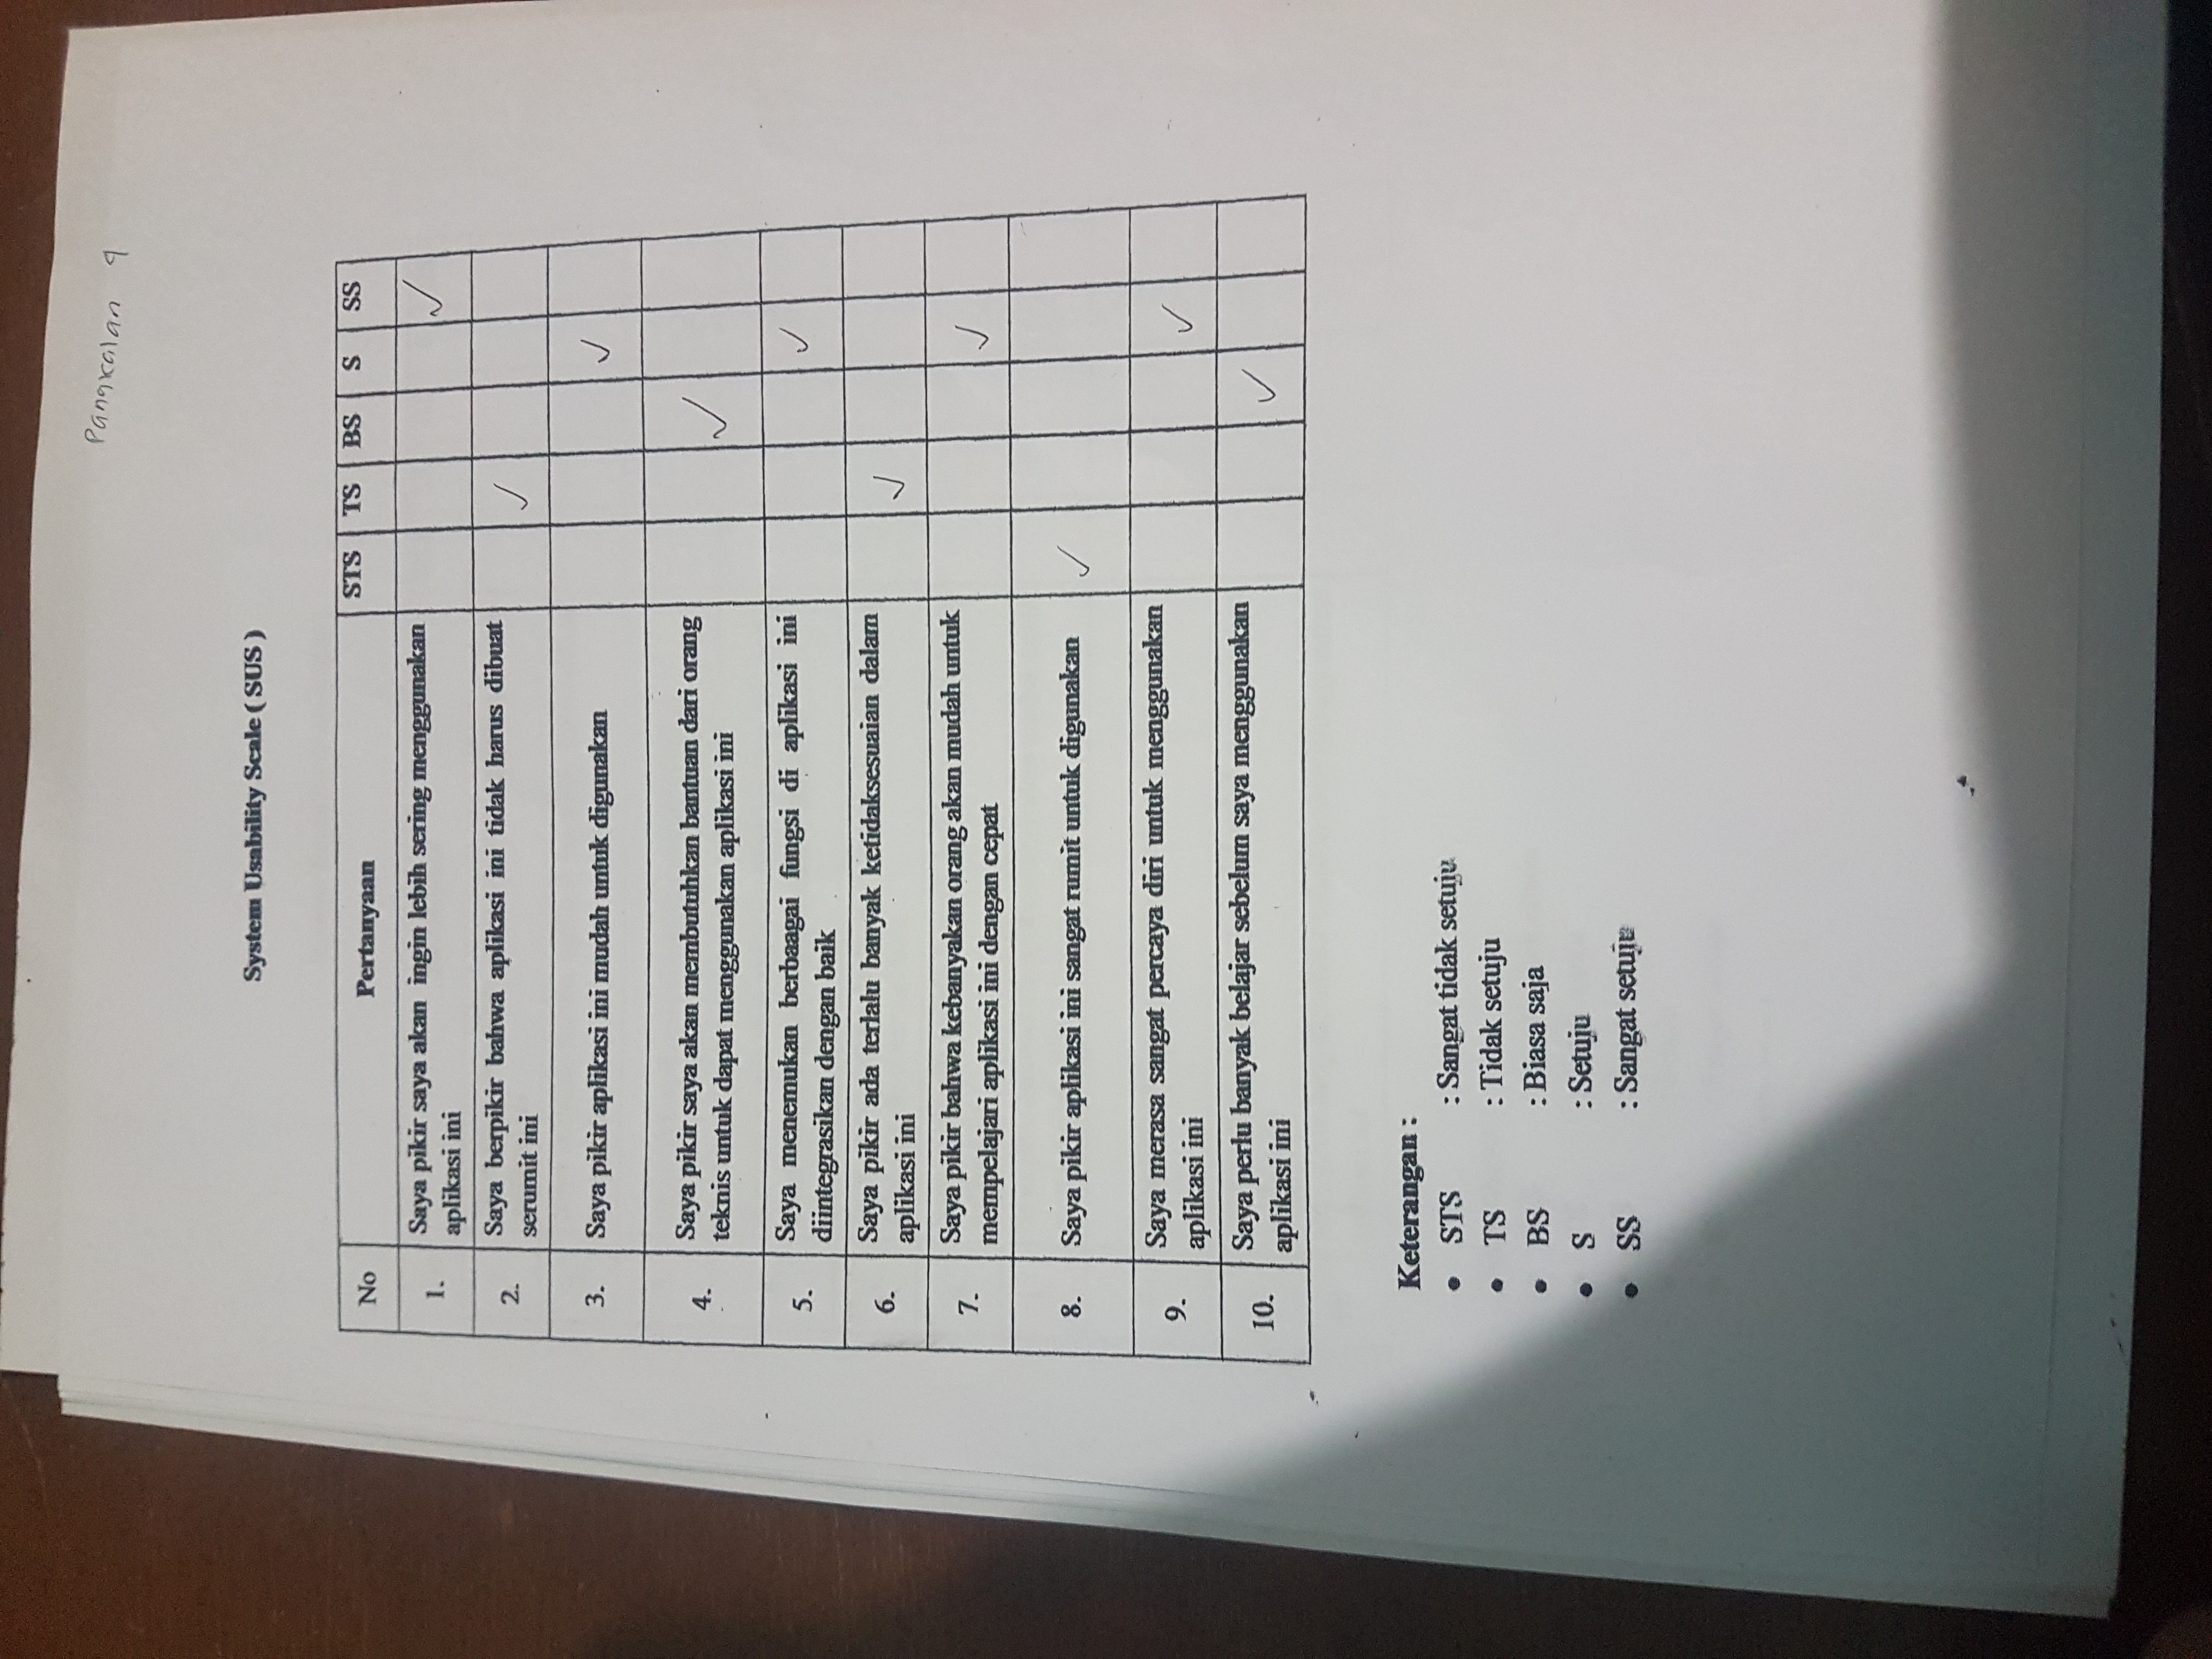
\includegraphics [width = 17cm,angle=-90]{gambar/pengujian/pangkalan4}
\end{figure}
\begin{figure}[H]
	\center
	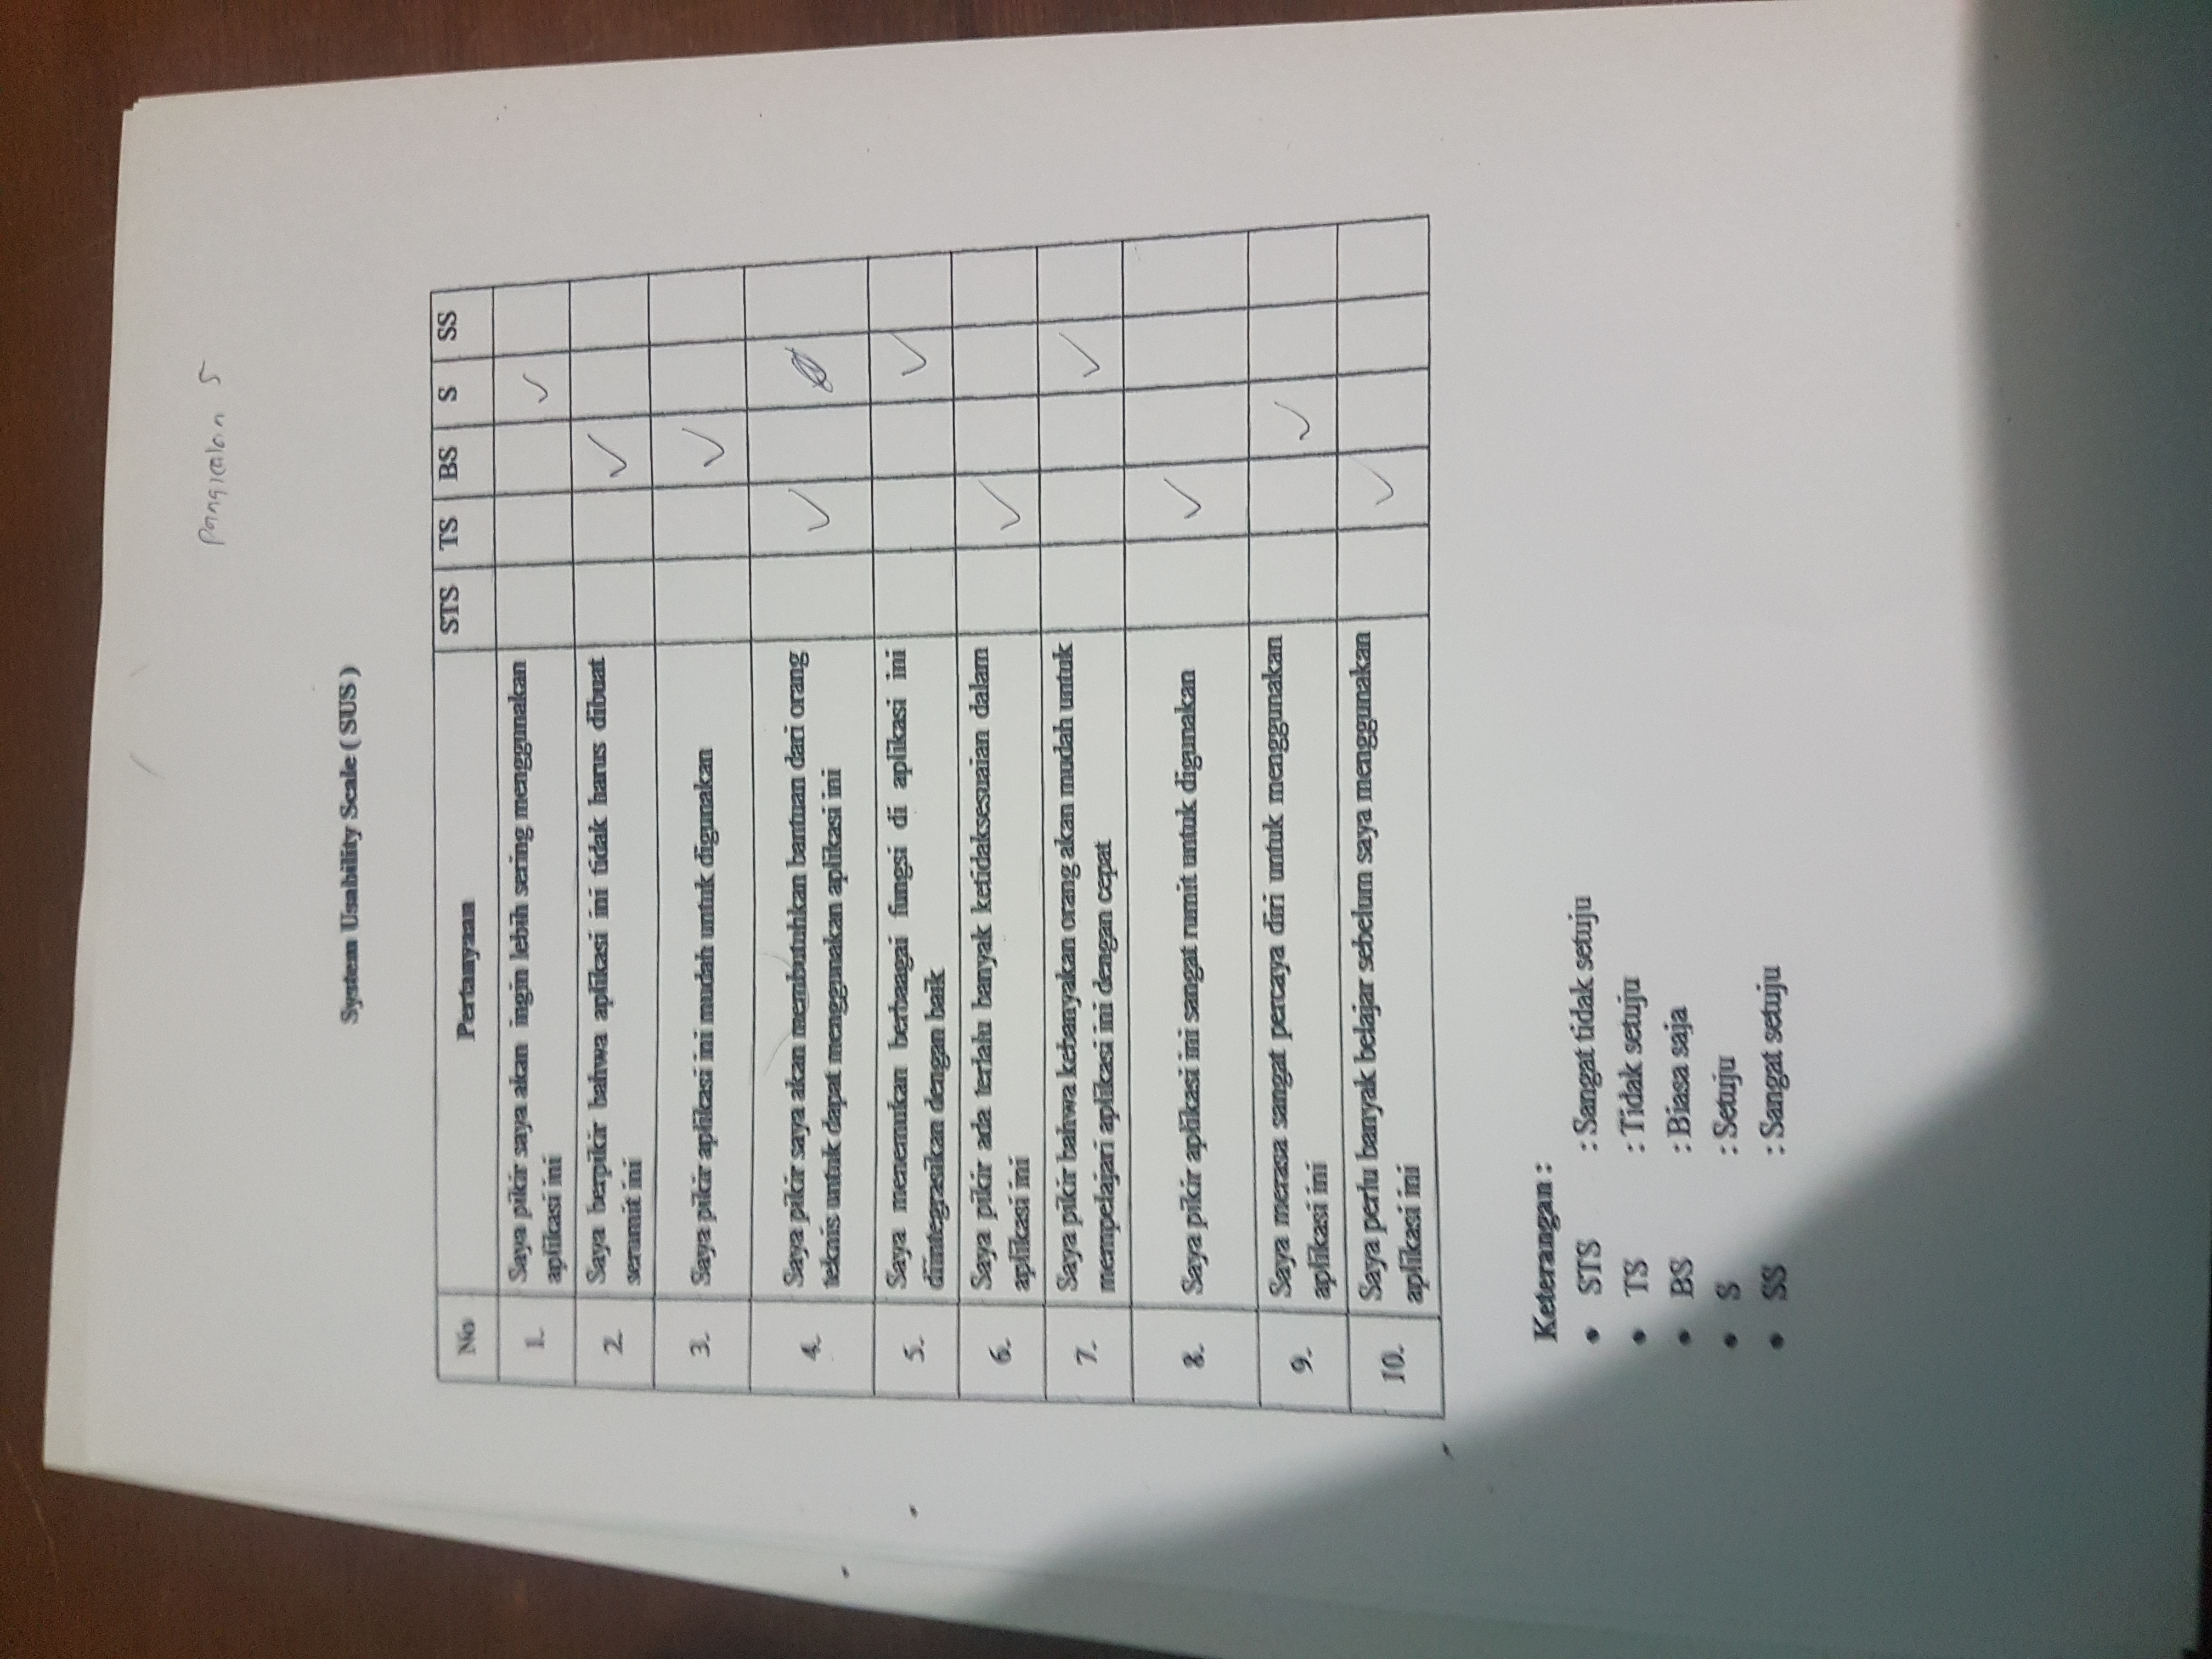
\includegraphics [width = 17cm,angle=-90]{gambar/pengujian/pangkalan5}
\end{figure}
\begin{figure}[H]
	\center
	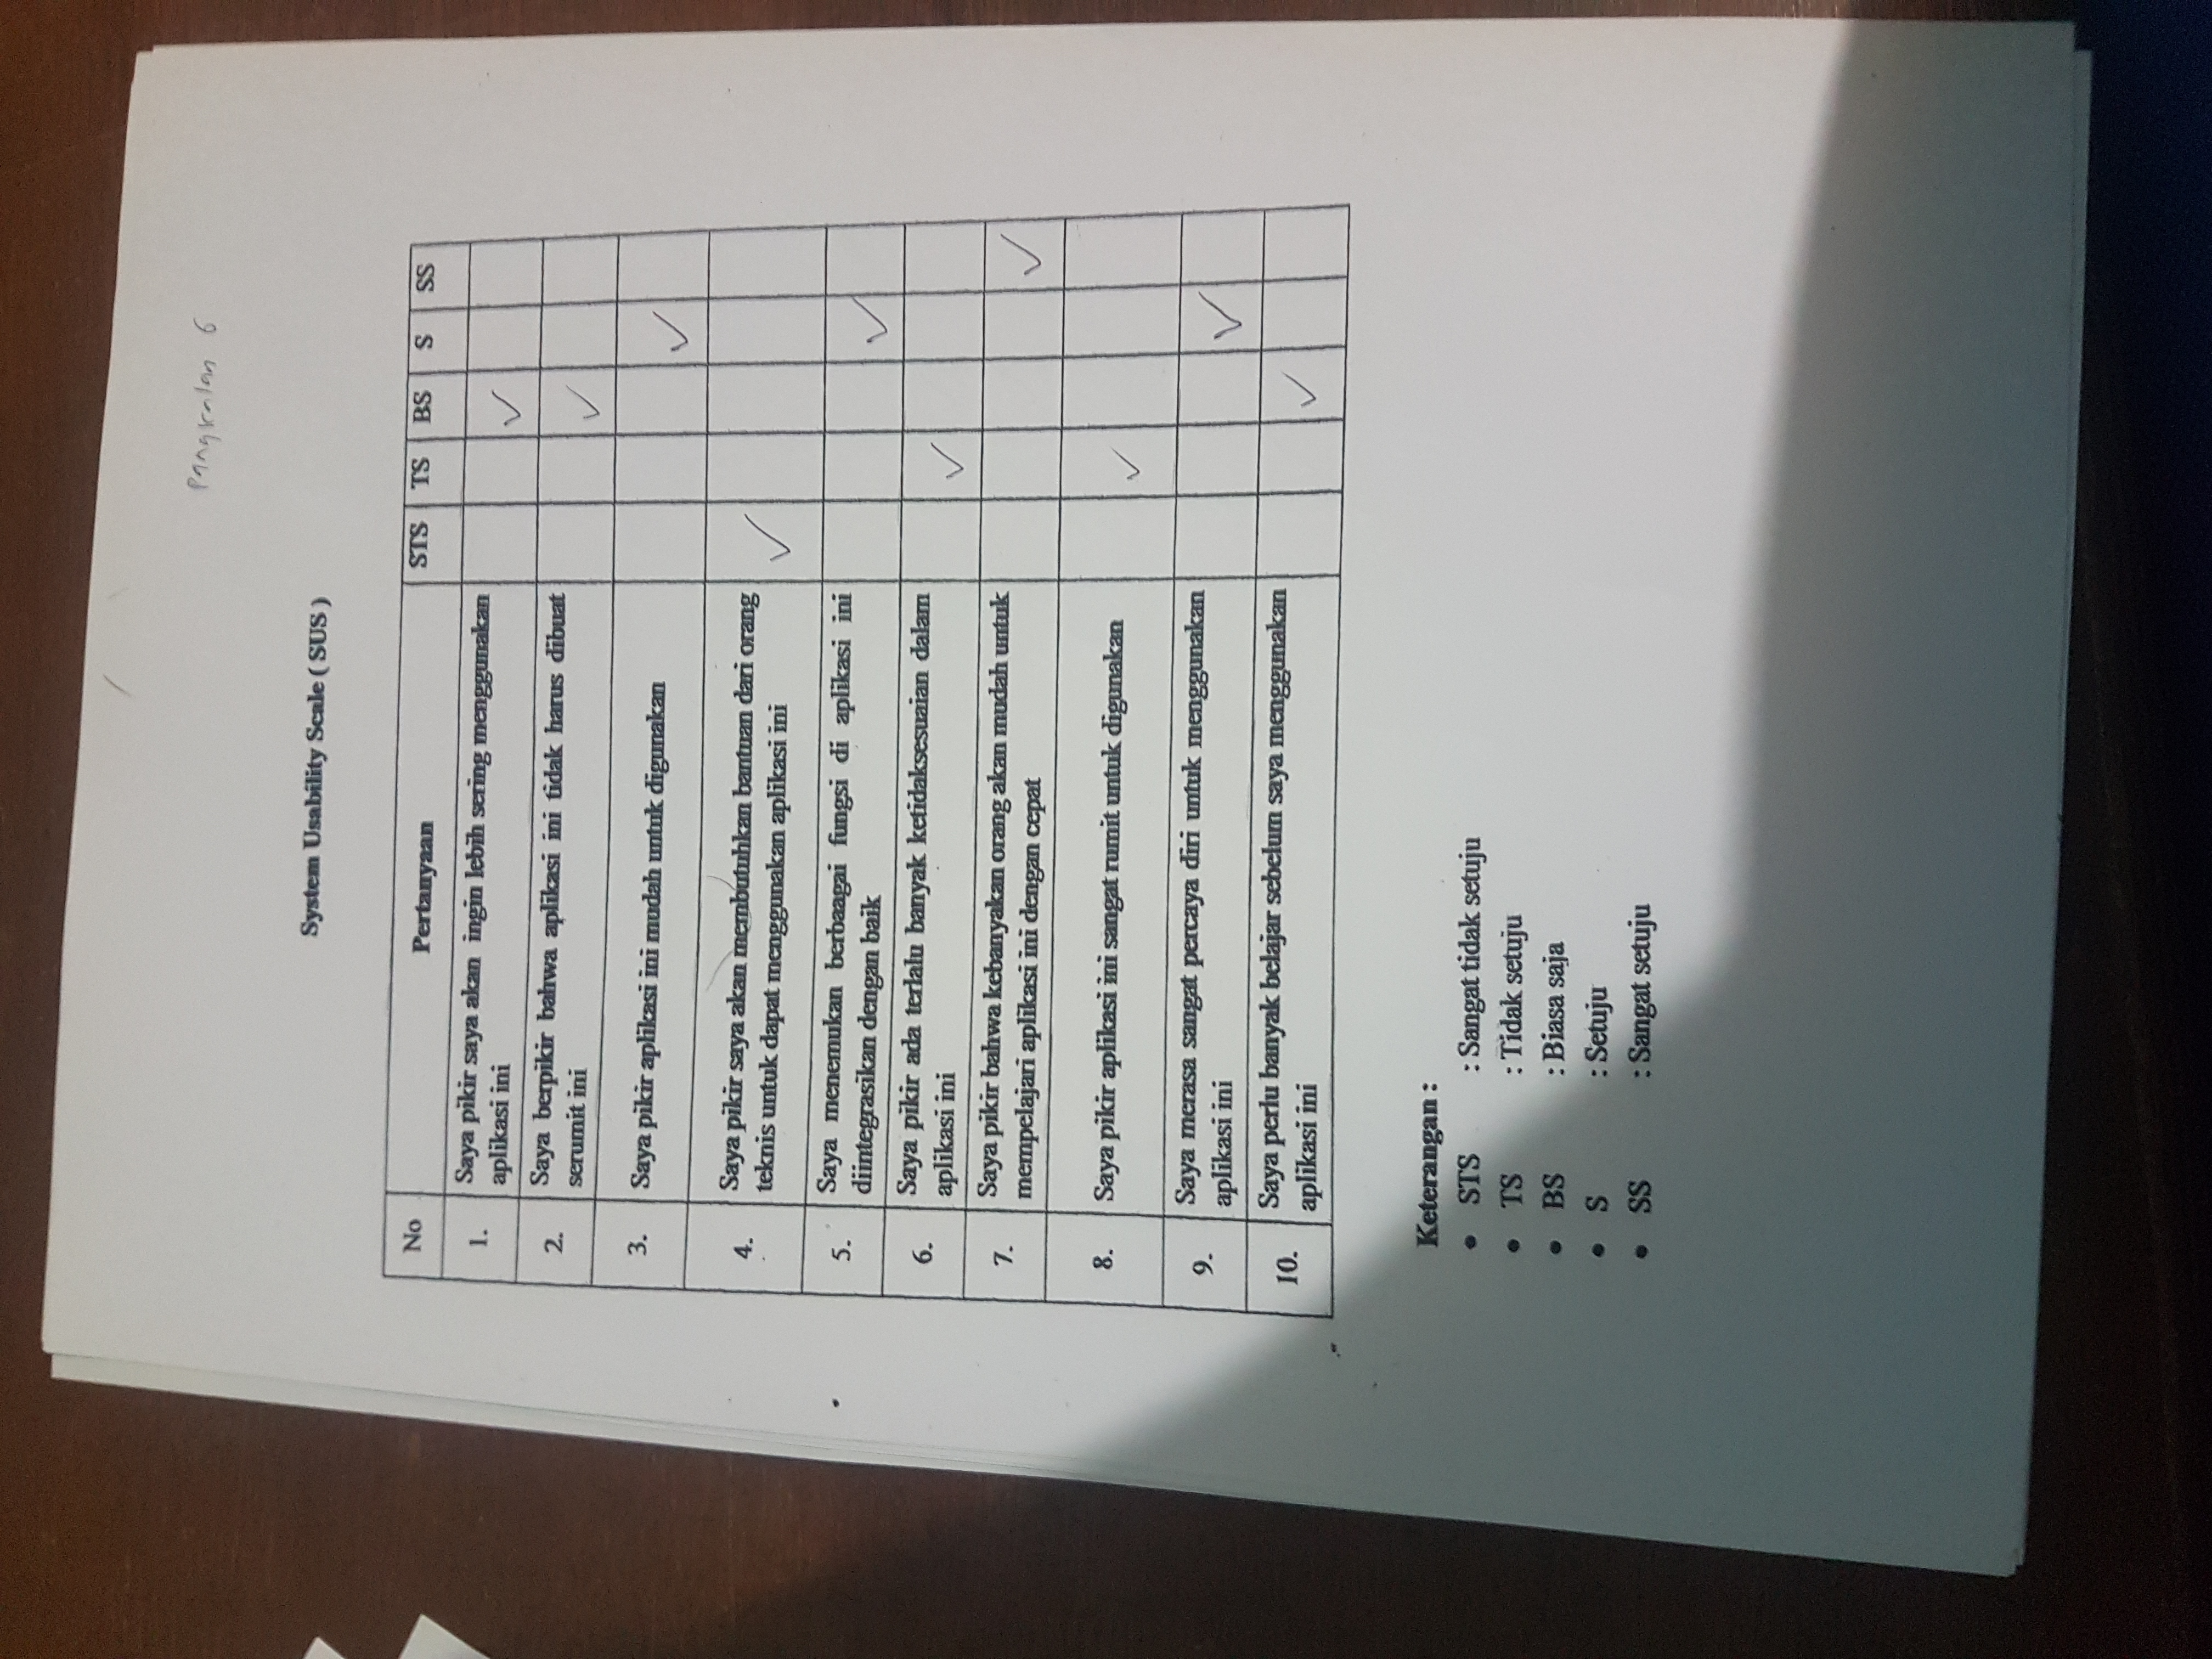
\includegraphics [width = 17cm,angle=-90]{gambar/pengujian/pangkalan6}
\end{figure}
\begin{figure}[H]
	\center
	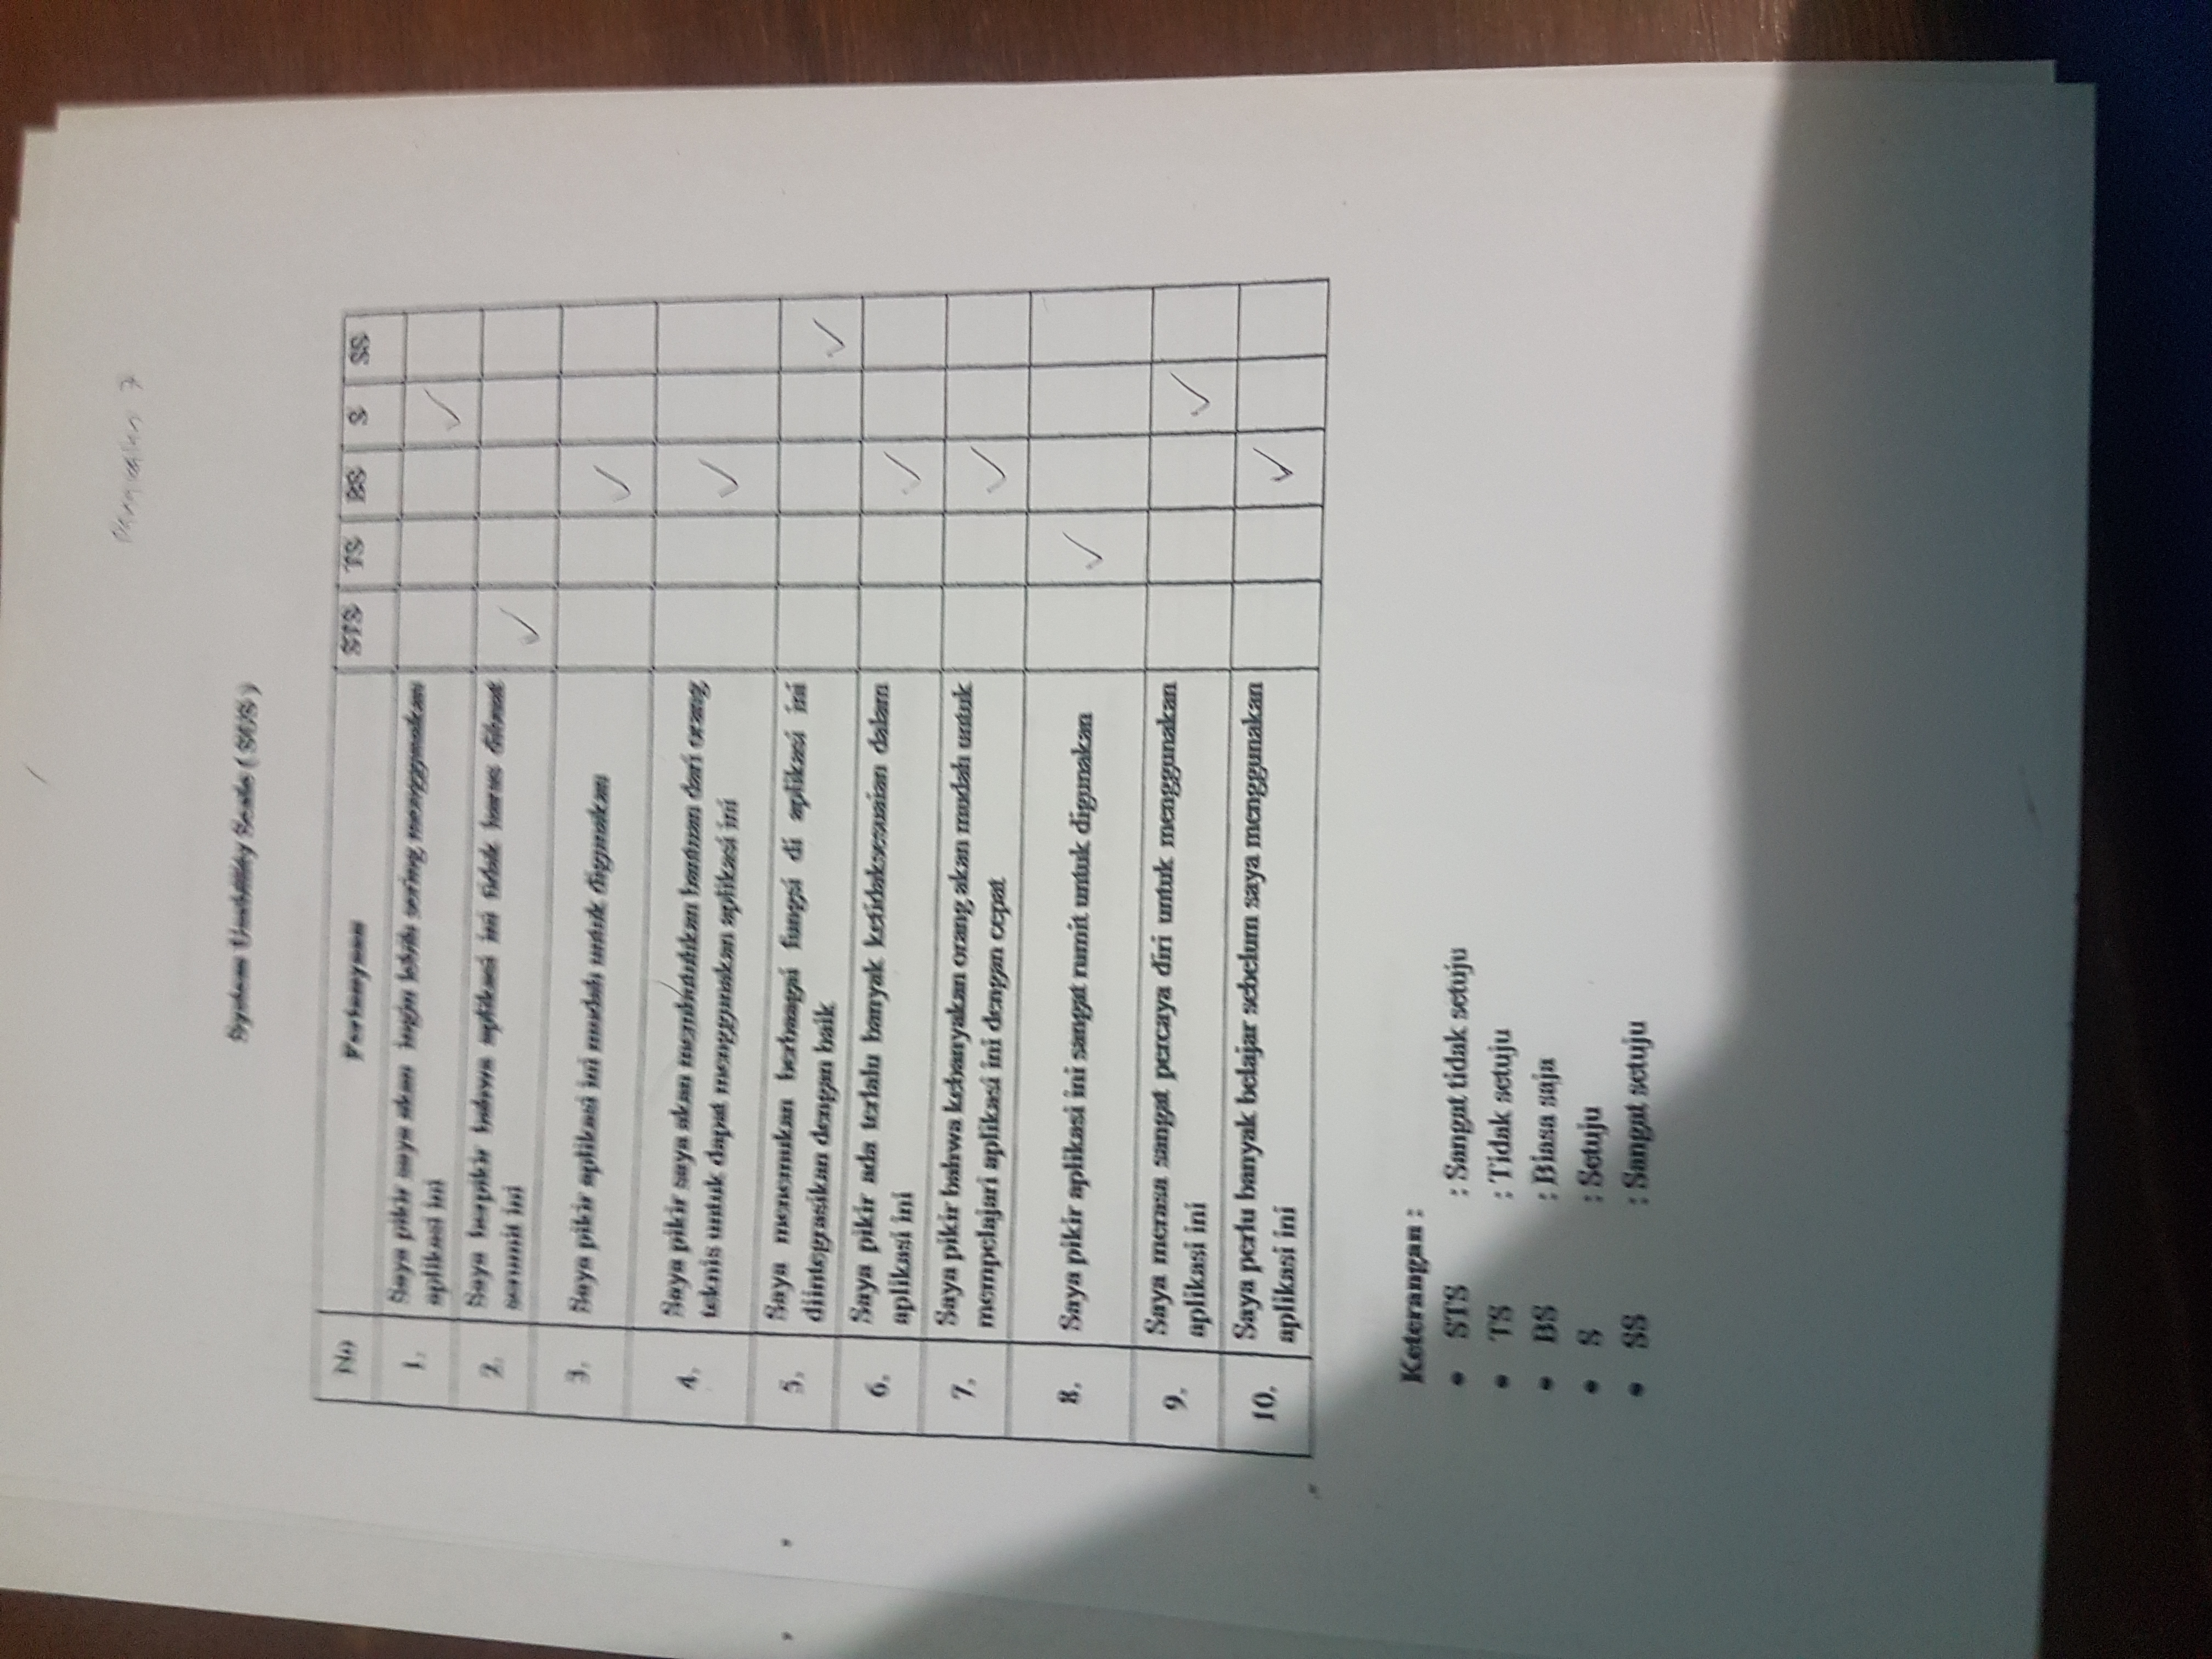
\includegraphics [width = 17cm,angle=-90]{gambar/pengujian/pangkalan7}
\end{figure}
\begin{figure}[H]
	\center
	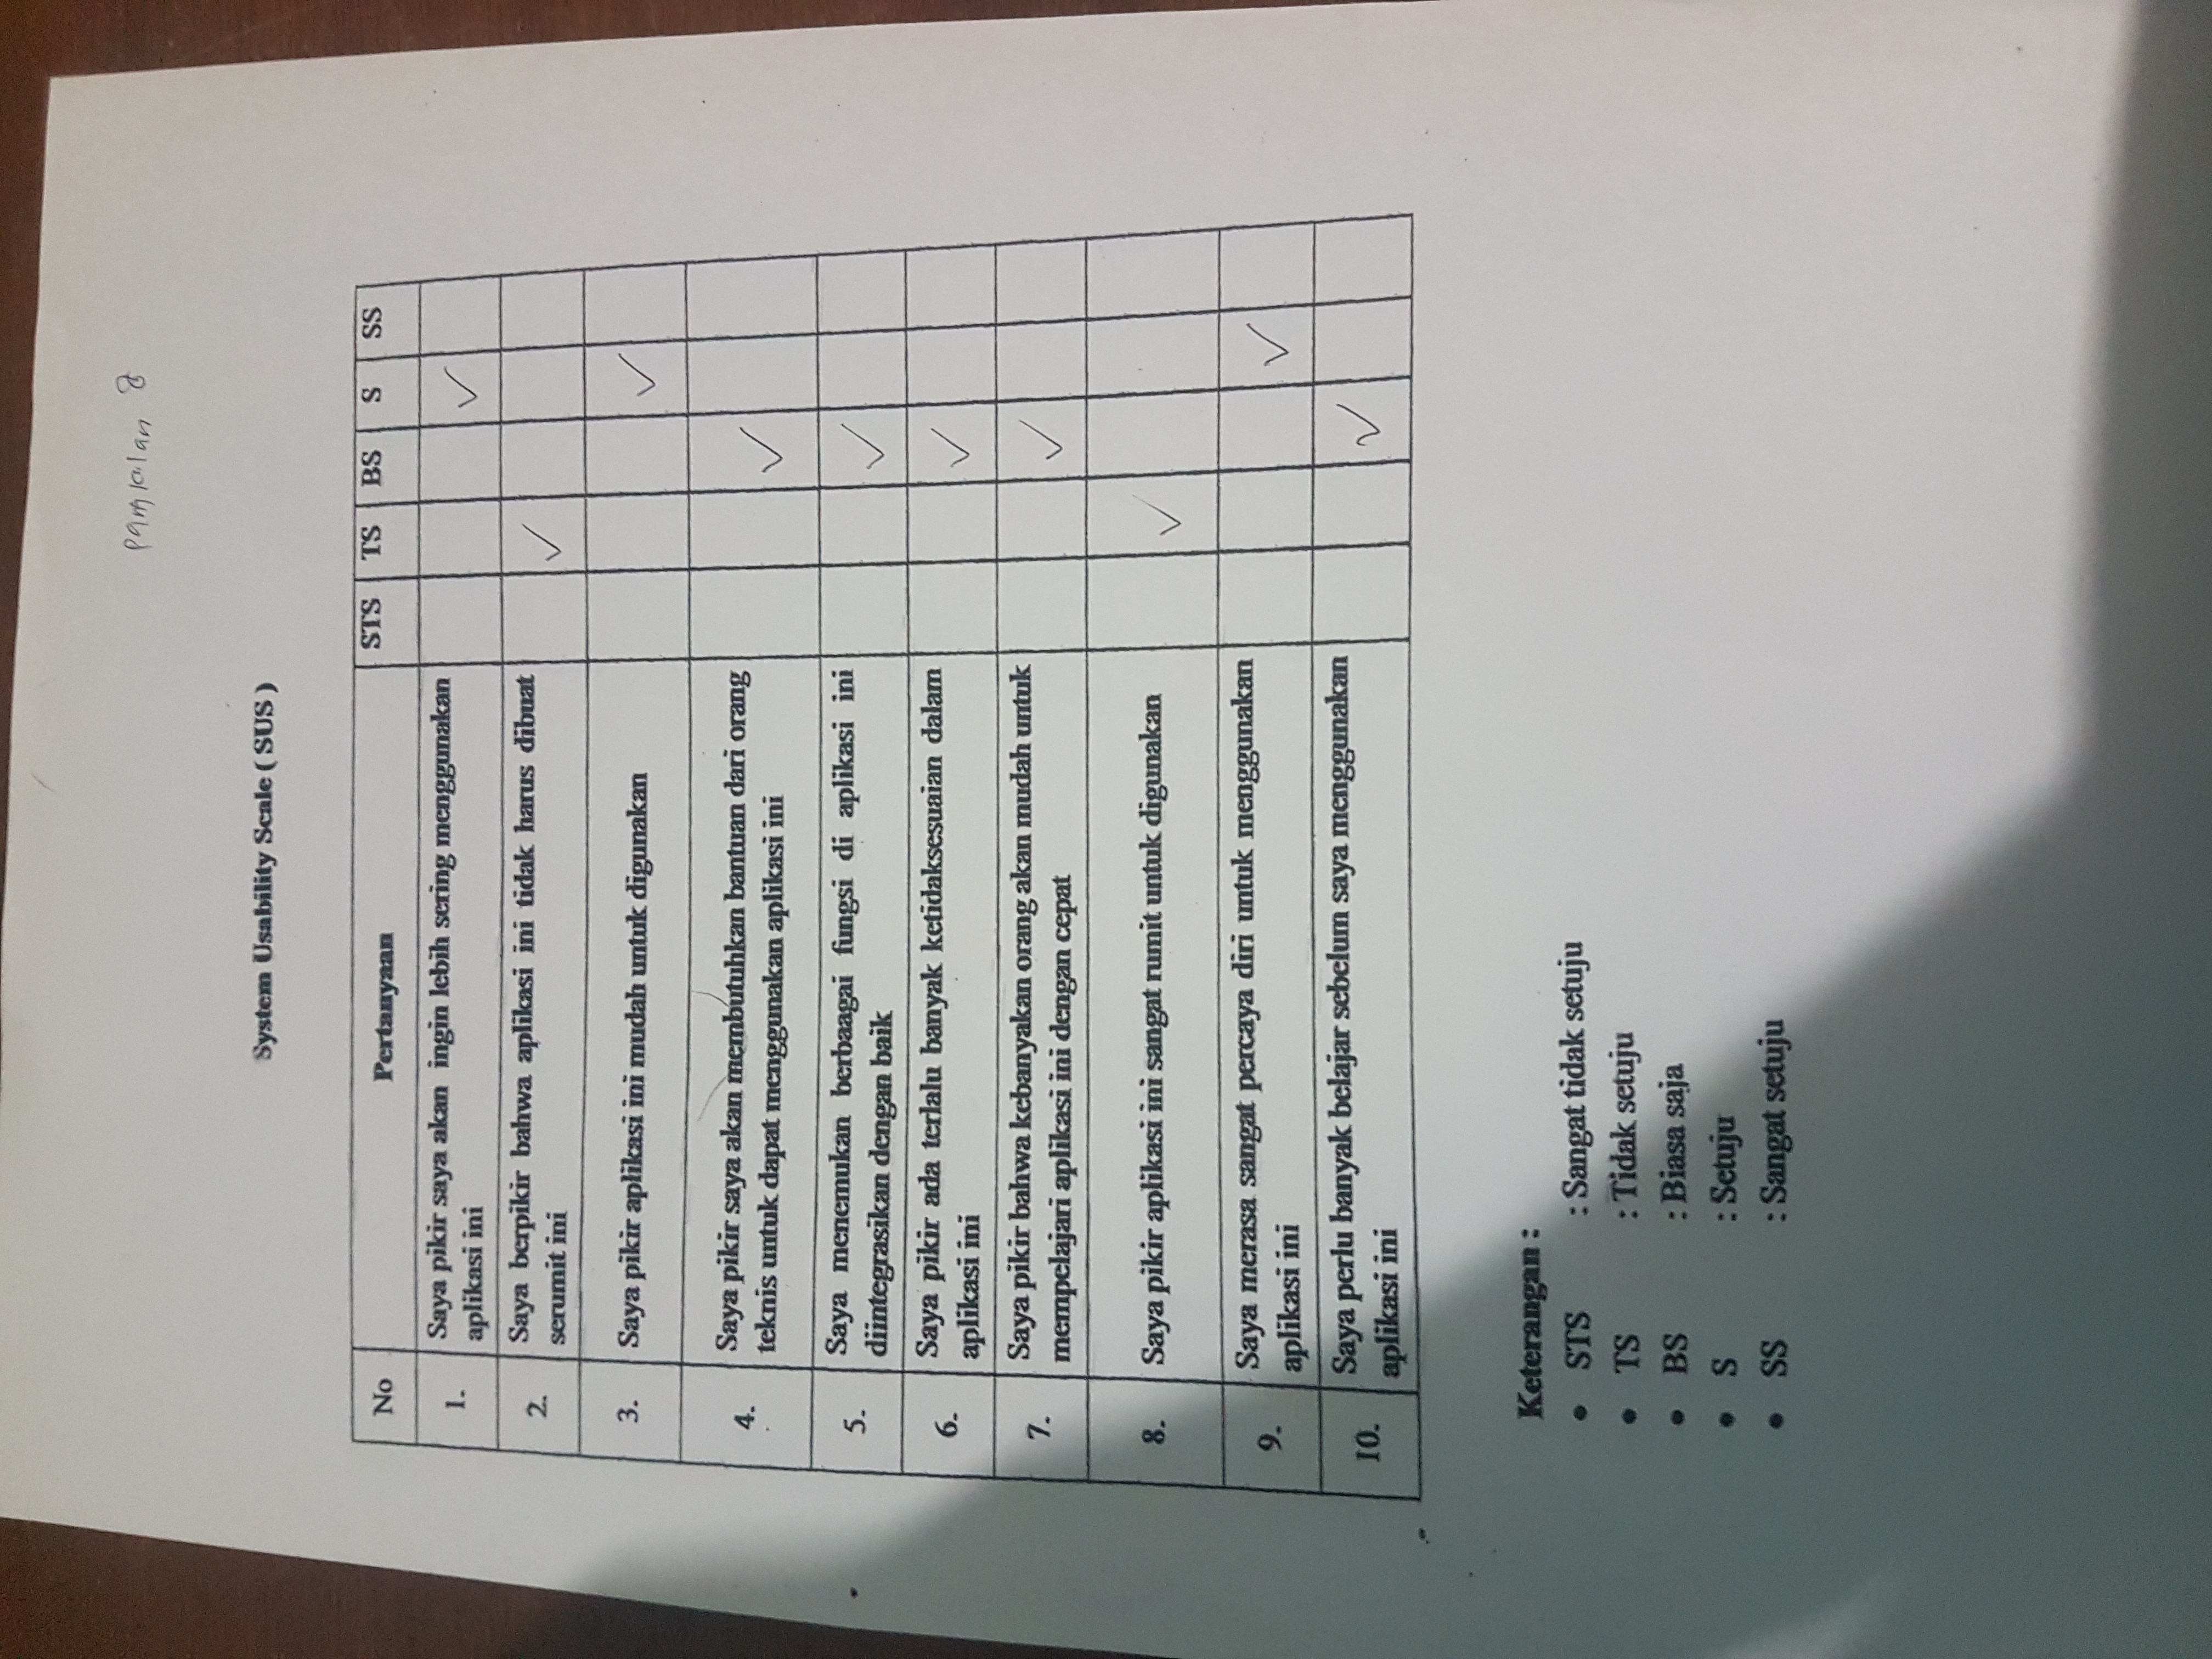
\includegraphics [width = 17cm,angle=-90]{gambar/pengujian/pangkalan8}
\end{figure}

%-----------------------------------------------------------------------------%
\addcontentsline{toc}{chapter}{LAMPIRAN 3}
\chapter*{Lampiran 3}
\newappendix{Lampiran 3. Foto Pengujian \textit{Usability}}
\begin{figure}[H]
	\center
	\includegraphics [width = 15cm, angle=-90]{gambar/pengujian/uji1}
\end{figure}

\begin{figure}[H]
	\includegraphics [width = 15cm]{gambar/pengujian/uji2}
	\vspace{2cm}
	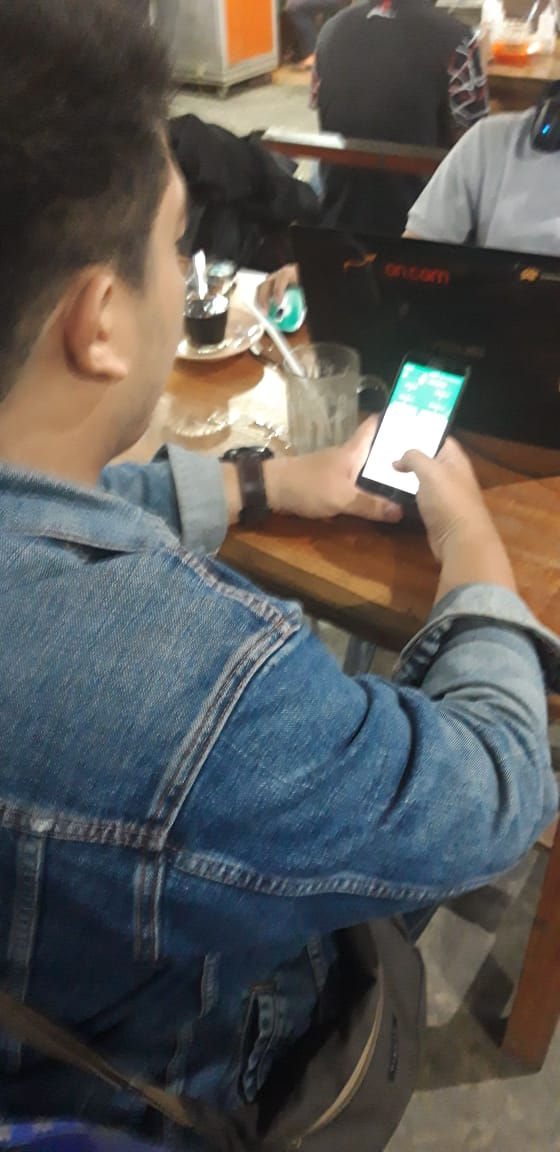
\includegraphics [height = 12cm]{gambar/pengujian/uji3}
\end{figure}


%-----------------------------------------------------------------------------%

%Lampiran 4 Laporan Usability

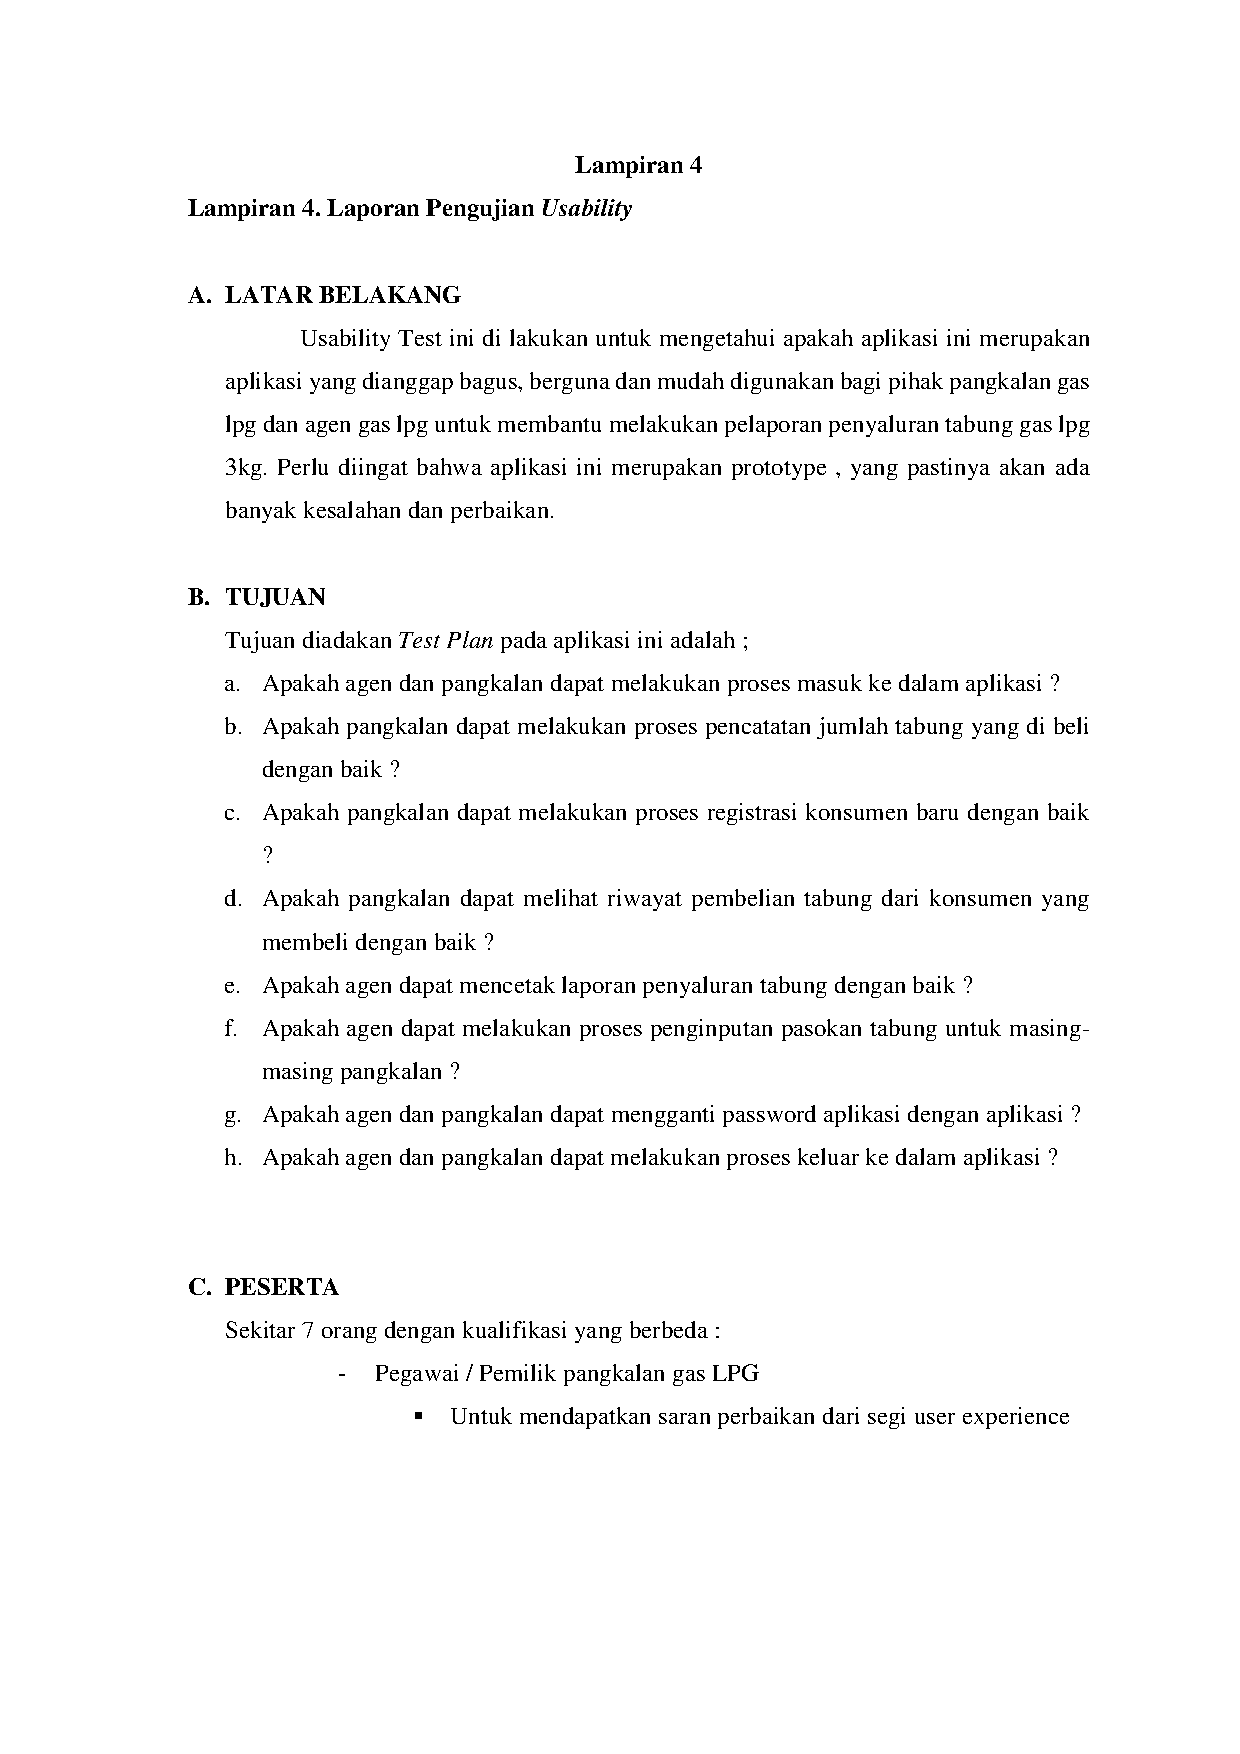
\includepdf[pages=1,scale=.8,pagecommand={
	\addcontentsline{toc}{chapter}{LAMPIRAN 4} 
	\chapter*{Lampiran 4}
	\newappendix{Lampiran 4. Laporan Hasil Pengujian \textit{Usability}}
},linktodoc=true]{laporan_usability}
\includepdf[pages=2-,scale=.8,pagecommand={},linktodoc=true]{laporan_usability}
